\chapter{Combinatorische Schakelingen (Schakelingen zonder geheugen)}
\chplab{combinatoric}
\chapterquote{Zelfs al zou er niets nieuws geschapen worden, dan is er nog altijd een nieuwe combinatie.}{Henry Ford, Amerikaans automobielfabrikant (1863-1947)}

\begin{chapterintro}
Nu we de basis van het bouwen van digitale circuits onder de knie hebben, en de fysische beperkingen hiervan kennen, kunnen we nuttige schakeling zoals optellers en vergelijkers ontwikkelen. \gtermen{Combinatorische Schakelingen}{Schakelingen waarbij een bitvector aan de uitgangen uitsluitend wordt bepaald aan de hand van een bitvector aan de ingangen. Er zijn met andere woorden geen geheugencomponenten en de schakeling houdt bijgevolg geen toestand bij. Onder combinatorische schakelingen vinden we bijvoorbeeld optellers, vergelijkers en multiplexers.} zijn schakelingen waarbij een bitvector aan uitgangen uitsluitend bepaald wordt aan de hand van een bitvector aan ingangen. We kunnen dus stellen dat het circuit een functie $\vec{f}(\vec{x})$ berekent. In \secref{synthese} werd reeds een manier voorgesteld om voor een gegeven functie tot een schakeling van canonieke vorm te komen. In \secref{minimalisatie} zullen we kennis maken met technieken zien om deze implementaties verder te minimaliseren. In \secref{rekenkundig} en \secref{andereBasis} bespreken we de implementatie van enkele populaire combinatorische schakelingen.
\end{chapterintro}

\minitoc[n]

\section{Minimaliseren van logische functies}
\seclab{minimalisatie}

In deze sectie geven we eerst een motivatie waarom het minimaliseren van implementaties een belangrijke taak is. Daarna tonen we een methode om op effici\"ente wijze een minimale implementatie te realiseren. We zullen ook een aantal uitbreidingen op deze methode beschouwen.

\subsection{Waarom minimaliseren}
\ssclab{whyMinimize}
In deze sectie zullen we als leidend voorbeeld schakelingen ontwerpen voor de worteltrekking en $7$-segment display in een minimale implementatie. Streven naar een minimalisatie is een algemeen probleem en is vergelijkbaar met optimalisatie in de informatica. Minimalisatie levert niet enkel snellere doorvoer op. Hieronder sommen we de meest courante voordelen op, samen met hun metriek:
\begin{itemize}
\item Minimaliseren van de \termen{kostprijs}. Afhankelijk van de realisatie hanteren we hiervoor twee metrieken: Voor CMOS verfijnen we hiervoor de oorspronkelijke formule van de kostprijs uit \eqnref{kosten}. En bekomen:

\begin{equation}
\mbox{kostprijs}=\displaystyle\sum_{\tiny\begin{array}{c}\mbox{alle}\\\mbox{poorten}\end{array}}{\funm{kostprijs}{\mbox{poort}}}
\eqnlab{kostenCmos}
\end{equation}

De kostprijs van een poort wordt dan bepaald met volgende formule:

\begin{equation}
\funm{kostprijs}{\mbox{poort}}=\acclguard{
\mbox{fan-in}&\mbox{if}\;\mbox{poort}\in\accl{\mbox{INV},\mbox{NAND},\mbox{NOR},\mbox{AOI},\mbox{OAI}}\\
\mbox{fan-in}+1&\mbox{if}\;\mbox{poort}\in\accl{\mbox{AND},\mbox{OR}}
}
\eqnlab{kostenCmosPoort}
\end{equation}

We zien dus dat alle \gtermen{inverterende poorten}{Poorten waar conceptueel op het einde een inverter staat. Inverterende poorten zijn INV, NAND, NOR, AOI en OAI.} relatief $1$ goedkoper zijn dat de \gtermen{niet-inverterende poorten}{Poorten waar conceptueel op het einde geen inverter staat. Niet-inverterende poorten zijn AND en OR.}. Bij een FPGA bepalen we de kostprijs aan de hand van het aantal logische cellen:

\begin{equation}
\mbox{kostprijs}=\#\mbox{LB's}
\end{equation}

Uiteraard dient hierbij de kanttekening gemaakt te worden, dat niet voor elk gegeven aantal logische cellen, er een FPGA bestaat. Indien er voldoende logische cellen op de FPGA aanwezig zijn, is de kostprijs dan ook van minder belang. We zullen immers toch dezelfde FPGA gebruiken.
\item Snelheid: We maximaliseren de snelheid door de maximale vertraging te minimaliseren. Deze vertraging is afhankelijk van de poorten in het \gtermen{kritische pad}{Een pad van ingang tot uitgang in een schakeling die de grootste vertraging heeft. Het is mogelijk dat een schakeling verschillende kritische paden heeft, al deze paden hebben dan dezelfde (theoretische) vertraging.}. Het kritische pad is een pad van de ingang naar de uitgang met de grootste vertraging. Deze vertraging is afhankelijk van twee parameters:
\begin{itemize}
\item Vertraging van de poorten: een poort heeft tijd nodig om bij verandering van de ingang ook de uitgang te veranderen. Deze vertraging is afhankelijk van de technologie en evenredig met de fan-in. We zullen deze benaderen met de volgende formule:

\begin{equation}
\funm{vertraging}{\mbox{poort}}=\acclguard{
0.6+0.4\cdot\mbox{fan-in}&\mbox{if}\;\mbox{poort}\in\accl{\mbox{INV},\mbox{NAND},\mbox{NOR},\mbox{AOI},\mbox{OAI}}\\
1.6+0.4\cdot\mbox{fan-in}&\mbox{if}\;\mbox{poort}\in\accl{\mbox{AND},\mbox{OR}}
}
\eqnlab{speedPoort}
\end{equation}

Deze formule toont dus dat opnieuw de fan-in een belangrijke factor is, en dat niet-inverterende poorten opnieuw een nadeel hebben tegenover inverterende poorten.
\item (capacitieve) belasting: dit hangt hoofdzakelijk af van de geometrische implementatie van de printplaat. Deze vertraging is dan ook zeer moeilijk te berekenen en wordt niet beschouwd.
\end{itemize}

We berekenen dan de formule met volgende formule:

\begin{equation}
\mbox{vertraging}=\displaystyle\sum_{\tiny\begin{array}{c}\mbox{kritisch}\\\mbox{pad}\end{array}}{\funm{vertraging}{\mbox{poort}}}
\eqnlab{speed}
\end{equation}

\end{itemize}

\subsection{Hoe minimaliseren?}
Om te minimaliseren hebben we een methode nodig. Deze methode manipuleert de logische uitdrukking van $\fun{\vec{f}}{\vec{x}}$ tot een uitdrukking die equivalent maar voordeliger is, rekening houdend met de metrieken van \eqnref{kostenCmos} en \eqnref{speed}.

\paragraph{}
Een probleem is echter dat er geen methodes bestaan die ons een reeks manipulaties voorstellen, waardoor we altijd tot de meest optimale implementatie komen. We moeten dus bijgevolg methodes bedenken waarmee we in staat zijn een redelijk optimale oplossingen te bekomen. Hiervoor zullen we methodes gebruiken zoals Karnaugh-kaarten. Computers bieden bovendien de mogelijkheid een groot aantal implementaties te simuleren. Bij een groot probleem volstaat ook deze rekenkracht niet meer om tot de beste implementatie te komen\footnote{Wat is \"uberhaupt de beste oplossing, in veel gevallen zal de ene metriek verbeteren ten koste gaan van de tweede.}.

\subsection{Karnaugh-kaarten}
\gtermen{Karnaugh-kaarten}{De projectie van een $N$-kubus in twee dimensies. Karnaugh-kaarten vormen een visueel hulpmiddel bij de synthese van een combinatorische schakeling voor een gegeven booleaanse functie met twee lagen.} of \stermen{K-kaarten}{Karnaugh-kaarten} proberen het aantal nutteloze ingangen tot een minimum te beperken. Het is een visueel hulpmiddel dat gebruik maakt van een vermogen waar mensen goed in zijn: het herkennen en begrijpen van patronen. De basis van een Karnaugh-kaart is dan ook de waarheidstabel. In een waarheidstabel kunnen we vaak door bepaalde rijen te beschouwen verbanden zien.
%Zo zien we in de waarheidtabel op figuur \ref{fig:sevenSegmentDisplay} dat $e=0$ als $w=1$. Uiteraard blijft er onduidelijkheid waarom $e=0$ als $\left(w,x,y,z\right)=\left(0,1,0,0\right)$. Toch kunnen we met dergelijke patronen de expressie al behoorlijk optimaliseren. Zo kunnen we voor $e$ al een expressie maken van de vorm $e=(\mbox{NOT }w)\mbox{ AND }\varphi$ met $\varphi$ een nog onbekende logische expressie. We weten immers dat indien $w=1$ er een 0 aan de ingang van de AND poort verschijnt. Een AND met aan minstens \'e\'en ingang een 0 is per definitie 0. We hebben dus het probleem kunnen reduceren met het zoeken naar een specifiek patroon.

\paragraph{N-kubus}
Karnaugh-kaarten zijn niets anders dan de projectie van waarheidstabellen naar een tweedimensionele figuur. Wanneer we een waarheidstabel met $N$ variabelen beschouwen, kunnen we dit in $N$ dimensies projecteren op een zogenoemde \termen{$N$-kubus}. Een $N$-kubus construeren we door booleaanse punten te beschouwen in $N$ dimensies: $\accl{0,1}^n$; en vervolgens bogen te trekken tussen elke twee punten waar er hoogstens \'e\'en variabele verschilt. De \gtermen{buren}{De buren van een knoop $k$ in een graaf is de verzameling van knopen zodat er een boog bestaat tussen $k$ en de knoop in kwestie.} van een knoop $K$ is de verzameling knopen waarvoor er een boog bestaat van of naar $K$. \figref{nCube} toont $N$-kubussen voor $1$ tot $4$ dimensies.

\begin{figure}[htb]
\centering
\subfigure[1D]{\importtikz{kubus1d}}
\subfigure[2D]{\importtikz{kubus2d}}
\subfigure[3D]{\importtikz{kubus3d}}
\subfigure[4D]{\importtikz{kubus4d}}
\caption{N-kubus voor dimensies $1$ tot $4$.}
\figlab{nCube}
\end{figure}

Elke knoop van de $N$-kubus beschrijft bitvector van waarden aan de ingang. We kunnen dan vervolgens op deze knooppunten de waarde die we aan de uitgang verwachten plaatsen. Buren zijn cruciaal, indien de uitgang niet verandert tussen twee buren, kunnen we zeggen dat de veranderde ingangsbit irrelevant is voor de uitgang.

\paragraph{Karnaugh-Kaarten}
Zoals eerder gesteld zijn Karnaugh-kaarten zijn in feite niets anders dan 2D projecties van de hierboven beschreven $N$-kubus. De projectie van een $N$-kubus naar twee dimensies is eenvoudig voor $N\leq 2$: het is gewoon de $N$-kubus zelf. Vanaf dimensies hoger dan 2 wordt het moeilijker.

\importtikzfigure{nCubeKarnaugh}{Van $N$-kubus naar Karnaugh-kaart.}

\figref{nCubeKarnaugh} toont de overgang van een $3$-kubus naar de respectievelijke Karnaugh-kaart. Bij een $N$-kubus heeft elke toestand $N$ buren. Nochtans zien we op de figuur dat de linkse en rechtse toestanden slechts 2 buren hebben in plaats van 3. We moeten dan ook op een Karnaugh-kaart modulo rekenen: de linkse buur van het meest linkse veld is het rechtse veld. Hetzelfde geldt in de andere richtingen. Elke cel in de Karnaugh-kaart beschrijft een bepaalde configuratie aan de ingangen. Aan de rand van de Karnaugh-kaart noteren we de naam van deze ingangen, en duiden we met een lijn bij welke cellen deze ingang $1$ is. Voor cellen die niet omvat worden door deze lijn, zal de bijbehorende ingang op dat moment $0$ zijn. Zo komt de cel linksboven op de figuur overeen met de configuratie $\tupl{x,y,z}=\tupl{0,0,0}$: alle ingangen zijn $0$. De cel rechtsonder komt dan weer overeen met de configuratie $\tupl{x,y,z}=\tupl{1,1,0}$: alleen ingang $z$ legt in dat geval een $0$ aan.

\begin{figure}[hbt]
\centering
\subfigure[1D]{\importtikz{karnaugh1d}}
\subfigure[2D]{\importtikz{karnaugh2d}}
\subfigure[3D]{\importtikz{karnaugh3d}}
\subfigure[4D]{\importtikz{karnaugh4d}}
\subfigure[5D gespiegeld]{\importtikz{karnaughKaarten5DMirror}}
\subfigure[5D gekopieerd]{\importtikz{karnaughKaarten5DCopy}}
\caption{Karnaugh-kaarten voor verschillende dimensies met binaire waarden.}
\figlab{karnaughKaarten}
\end{figure}

\figref{karnaughKaarten} toont Karnaugh-kaarten voor een verschillend aantal variabelen. In de cellen staat de decimale waarde van de ingang die deze cel vertegenwoordigt. Daarvoor gebruiken we de variabelen in de volgende volgorde: $\tupl{v,w,x,y,z}$. We kunnen in principe blijven uitbreiden. Vanaf zes dimensies wordt het echter moeilijk om nog patronen te herkennen. Karnaugh-kaarten hebben bijgevolg maar een beperkt vermogen.

\paragraph{Spiegelen of kopi\"eren}
Vanaf vijf dimensies groepeert men meestal cellen in rasters van $4\times 4$. Men gebruikt hierbij twee varianten: ofwel \gtermen{spiegelt}{Een manier om Karnaugh-kaarten voor te stellen indien het aantal dimensies stijgt boven de vier. In dat geval worden twee $4\times 4$ rasters beschouwd. Het tweede raster spiegelt de variabelen over de as tussen de twee rasters.} men \'e\'en van de twee tabellen zoals op \figref{karnaughKaarten5DMirror}, ofwel zijn de tabellen exacte \gtermen{kopies}{Een manier om Karnaugh-kaarten voor te stellen indien het aantal dimensies stijgt boven de vier. In dat geval worden er twee $4\times 4$ rasters beschouwd. Beide rasters gebruiken dezelfde positionering van de variabelen.} (op de waarde van \'e\'en enkele variabelen na) zoals op \figref{karnaughKaarten5DCopy}. Het spiegelen van variabelen is intu\"itiever omdat dit consistent is met lagere dimensies.

\subsubsection{Optimaliseren met behulp van Karnaugh-kaarten}
Nu we weten wat een Karnaugh-kaart is, bespreken we een methode om een optimale implementatie uit deze Karnaugh-kaarten af te leiden. We introduceren eerst terminologie, daarna bespreken we het stappenplan van de methode in detail met een voorbeeld. Tot slot beschouwen we enkele uitbreidingen op dit stappenplan.

\paragraph{Terminologie}
Alvorens we aan het optimalisatiewerk kunnen beginnen, hebben we nood aan enige terminologie. Een \gtermen{implicant}{Een implicant is een productterm, zodat er minstens \'e\'en cel op de Karnaugh-kaart is die zelf $1$ is en waarvoor de functie - beschreven door deze productterm - ook $1$ is. De functie-waarde voor cellen die $0$ zijn op de Karnaugh-kaart horen ook $0$ te zijn. De cellen op de Karnaugh-kaart die $1$ zijn, hoeven niet - op \'e\'en cel na - een functie-waarde $1$ te hebben.} is een productterm zodat de functie die ontstaat uit deze productterm $1$ is voor minstens \'e\'en cel op de Karnaugh kaart, die zelf ook $1$ is. De priemimplicant dient ook $0$ te zijn voor de cellen op de Karnaugh-kaart die zelf ook $0$ zijn. Voor alle overige cellen op de Karnaugh-kaart maakt het niet uit of de functie $0$ of $1$. Deze definitie heeft nauwe banden met de 1-minterm, het verschil is dat bij een implicant niet alle variabelen aanwezig moeten zijn. Zo zien we op \figref{karnaughKaartenImplicanten} verschillende implicanten met een verschillend aantal variabelen. Bij $1$-minterm - zoals we bespraken in \sscref{1minterm} - zijn altijd alle variabelen aanwezig in het product. Een \gtermen{priemimplicant}{Een implicant die geen onderdeel is van een andere implicant met strikt minder variabelen.} is een implicant die geen onderdeel is van een andere implicant met strikt minder variabelen. De priemimplicanten van \figref{karnaughKaartenImplicanten} worden weergegeven op \figref{karnaughKaartenPriemimplicanten}. Zo zien we op de figuur dat de implicant $x_1\cdot x_2\cdot x_3\cdot x_4'$ geen priemimplicant is: de implicant $x_1\cdot x_3\cdot x_4'$ is immers altijd waar wanneer $x_1\cdot x_2\cdot x_3\cdot x_4'$ waar is, en bestaat uit minder variabelen. Een verdere uitbreiding is de \gtermen[essentiele priemimplicant]{essenti\"ele priemimplicant}{Een priemimplicant die voor \'e\'en cel in de Karnaugh-kaart $1$ bevat, en waar er geen enkele andere priemimplicant voor deze cel $1$ geeft.}, dit is een priemimplicant die minstens \'e\'en 1-minterm omvat die niet in een andere priemimplicant verweven zit. Visueel is dit een priemimplicant die minstens \'e\'en cel omvat met $1$; en er bestaat geen enkele priemimplicant die deze cel omvat. Tenslotte defini\"eren we nog de \gtermen{dekking}{Een verzameling van implicanten voor een gegeven functie (en bijbehorende Karnaugh-kaart) zodat voor elke cel waar de functie $1$ is, deze cel minstens wordt omvat door een implicant in de verzameling. Bovendien is er geen enkele cel waar de functie $0$ is die omvat wordt door een implicant in de verzameling.} of \stermen{cover}{dekking} als een verzameling van implicanten zodat voor elke cel waar functie $1$ is, deze cel door minstens \'e\'en implicant in de verzameling wordt omvat. Daarnaast mag geen enkele implicant een cel omvatten waar de functie $0$ is.

\begin{figure}[hbt]
\centering
\subfigure[Implicanten]{\importtikz{karnaughKaartenImplicanten}}
\subfigure[Priemimplicanten]{\importtikz{karnaughKaartenPriemimplicanten}}
\subfigure[Essenti\"ele priemimplicanten]{\importtikz{karnaughKaartenEssentielePriemimplicanten}}
\caption{Terminologie van een Karnaugh-kaart.}
\figlab{karnaughKaartTerminologie}
\end{figure}

\paragraph{Stappenplan}
We minimaliseren een functie met behulp van een Karnaugh-kaart in vier stappen, deze stappen zullen we in de volgende paragrafen bespreken:
\begin{enumerate}
 \item Maak de Karnaugh-kaart.
 \item Bepaal alle priemimplicanten.
 \item Bepaal alle essenti\"ele priemimplicanten.
 \item Zoek de minimale dekking.
\end{enumerate}
Daarna zullen we nog drie speciale gevallen bestuderen.

\paragraph{}
We bestuderen deze methode aan de hand van een voorbeeld. We zullen een schakeling synthetiseren die de functies $f$ en $g$ berekent. Functie $f$ geeft $1$ terug bij de getallen $0$, $1$, $3$, $5$, $7$, $8$, $10$, $11$, $14$ en $15$, en $0$ in de andere gevallen, $g$ is waar als de afgeronde vierkantswortel van het getal even is. De waarheidstabellen van deze functies staan in \tblref{karnaugh-example}.

\begin{table}
\centering
\importtabularsubtable{karnaugh-example1}{$f$}
\importtabularsubtable{karnaugh-example2}{$g$}
\caption{Waarheidstabellen voor de leidende voorbeelden.}
\tbllab{karnaugh-example}
\end{table}

\paragraph{Stap 1: maak de Karnaugh-kaart}
In de eerste stap bouwen we een Karnaugh-kaart op die de logische functie visueel weergeeft. We tekenen een Karnaugh-kaart met het juiste aantal ingangsvariabelen (zie \figref{karnaughKaarten}) en vullen vervolgens de uitgangswaarden voor \'e\'en bepaalde uitgang in op de respectievelijke plaatsen. per uitgang dienen we een afzonderlijke kaart op te maken: in elke cel dienen we net \'e\'en bit te plaatsen.

\importtikzfigure{karnaughKaartenVoorbeeldGetekend}{Ingevulde Karnaugh-kaarten voor de uitgangen van het leidend voorbeeld.}

Op \figref{karnaughKaartenVoorbeeldGetekend} staan de Karnaugh-kaarten voor de functies $f$ en $g$. De variabelen $\tupl{x_1,x_2,x_3,x_4}$ vormen de binaire voorstelling van het invoergetal\footnote{Volgens de little-endian conventie.}.

\paragraph{Stap 2: bepaal alle priemimplicanten}
De volgende stap is het bepalen van alle priemimplicanten van de Karnaugh-kaart. Visueel is een implicant niets anders dan een rechthoek zodat zowel de lengte en de breedte een lengte hebben van - mogelijk verschillende - machten van twee\footnote{Niet te verwarren met veelvouden van twee.}. Deze rechthoeken vallen ook onder de modulo-regel op een Karnaugh-kaart: een rechthoek kan dus beginnen op de meest rechtse kolom, en doorlopen tot de meest linkse, zodat de kolommen in het midden worden overgeslagen. Een priemimplicant is een rechthoek zoals hierboven beschreven, maar waarbij een verdubbeling van de lengte of de breedte - in welke richting dan ook - niet langer mogelijk is. We kunnen priemimplicanten opsporen door eerst een cel met waarde $1$ te beschouwen, en dan telkens ofwel de lengte ofwel de breedte te verdubbelen tot dit niet langer mogelijk is. Dit is dus het geval wanneer er nullen bij een dergelijke verdubbeling in de rechthoek dreigen te komen liggen. doen. Indien er verschillende uitbreidingen mogelijk zijn, dienen al de uitbreidingen gevolgd te worden. \figref{karnaughKaartenVoorbeeldPriemimplicanten} toont de priemimplicanten voor de twee uitgangen van het leidend voorbeeld.

\importtikzfigure{karnaughKaartenVoorbeeldPriemimplicanten}{Karnaugh-kaarten met priemimplicanten van het leidend voorbeeld.}

\paragraph{Stap 3: Bepaal alle essenti\"ele priemimplicanten}
Nadat we de priemimplicanten bepaald hebben, zullen we uit deze verzameling de essenti\"ele priemimplicanten halen. Deze stap is eenvoudig: als een priemimplicant \'e\'en of meer cellen omvat die door geen enkele andere priemimplicant omvat worden, is dit een essenti\"ele priemimplicant. Deze implicanten zullen sowieso al tot de resulterende functie behoren. Op \figref{karnaughKaartenVoorbeeldEssentielePriemimplicanten} staan de essenti\"ele priemimplicanten voor $f$ en $g$. We zien duidelijk dat in beide gevallen de priemimplicanten onvoldoende zijn om de volledige functie te beschrijven daar er nog enen niet niet gedekt worden: dit komt omdat voor al deze cellen, er minstens twee priemimplicanten de cel bedekten.

\importtikzfigure{karnaughKaartenVoorbeeldEssentielePriemimplicanten}{Karnaugh-kaarten met essenti\"ele priemimplicanten van het leidend voorbeeld.}

\paragraph{Stap 4: Zoek de minimale dekking}
De essenti\"ele priemimplicanten zijn de goedkoopste manier om de cellen die ze dekken te implementeren, we zien echter dat dit in de meeste gevallen onvoldoende is om de volledige functie te beschrijven: er blijven cellen met waarde $1$ ongedekt. We dienen nog extra priemimplicanten toe te voegen om tot volledige dekking te komen. In het ideale geval doen we dit door alle mogelijke toevoegingen van priemimplicanten na te gaan. Dit is echter een erg arbeidsintensief proces. Men lost dit probleem dan ook meestal op met een ``\gtermen{gulzige strategie}{Een methode om een probleem op te lossen door het op te delen in verschillende beslissingen. Bij elke beslissing kiezen we de optie die ons onmiddellijk het meeste oplevert. Het is echter niet gezegd dat dit tot de uiteindelijke beste oplossing zal leiden, omdat een eerste beslissing er voor kan zorgen dat een tweede beslissing tot minder winst kan worden.}'' ofwel ``\stermen{greedy algorithm}{gulzige strategie}''. We beschouwen initieel de verzameling van essenti\"ele priemimplicanten, iedere iteratie voegen we de priemimplicant toe die het meeste aantal cellen dekt die tot dan toe ongedekt bleven. We stoppen op het moment dat de set van implicanten de volledige functie dekt. We illustreren dit proces op \figref{karnaughKaartenVoorbeeldGreedySearch} waarbij we elke iteratiestap tonen.

\importtikzfigure{karnaughKaartenVoorbeeldGreedySearch}{Werking van het greedy algoritme bij het leidend voorbeeld.}

\paragraph{Synthese}
Elk van de priemimplicanten die we geselecteerd hebben stelt het product voor van enkele variabelen. We implementeren de functie door de som te nemen van deze priemimplicanten. Voor het voorbeeld wordt dit dus:

\begin{equation}
\begin{array}{ll}
\acclguard{
\begin{array}{l}
f=x_2'x_3'x_4'+x_1'x_4+x_1x_3\\
g=x_1'x_3'x_4'+x_1'x_2'x_3x_4+x_2x_3x_4'+x_2x_3'x_4+x_1x_2x_3
}&\leaex
\end{array}
\end{equation}

\paragraph{Uitbreiding: Dambordpatroon}
Een patroon dat men vaak tegenkomt in Karnaugh-kaarten is het \gtermen{dambordpatroon}{Een veel voorkomend patroon waarbij wisselend in een ene rij men $0$ en $1$ tegenkomt, na enkele rijen wisselt het patroon naar $1$ en $0$. Wanneer het dambordpatroon voorkomt op een Karnaugh-kaart kan dit vaak effectief worden gerealiseerd met behulp van XOR poorten. De grootte van de vlakken bepaalt welke ingangen aan deze XOR poorten moeten worden gezet.}. Dit dambordpatroon hoeft niet noodzakelijk uit vierkanten te bestaan, rechthoeken zijn ook mogelijk. Indien we dit patroon met de klassieke Karnaugh-methode implementeren bekomen we een groot aantal priemimplicanten wat leidt tot dure implementaties, we kunnen in dat geval gebruik maken van XOR-operaties die we achter elkaar schakelen. Een aaneenschakeling van XOR-operaties impliceert een grotere vertraging maar heeft een grote invloed op de kostprijs. \figref{dambordpatronen} toont enkele dambordpatronen en hun implementatie met XOR-logica.

\importtikzfigure{dambordpatronen}{Voorbeelden van dambordpatronen in Karnaugh-kaarten.}

\paragraph{Uitbreiding: Don't cares}
\ssslab{dontcare}
In sommige gevallen dienen we slechts een beperkte set van invoer-configuraties te beschouwen. Stel bijvoorbeeld dat we een seven segment digitale display\footnote{Dit is een verzameling leds die zo georganiseerd is dat we met zeven leds, alle cijfers van $0$ to $9$ kunnen weergeven.} implementeren die getallen van $0$ tot en met $9$ voorstelt. In dat geval hebben we vier ingangen nodig. Maar we zullen bijvoorbeeld nooit de configuratie $1011_2=11_{10}$ aan de ingang tegenkomen. Er is echter wel een plaats gereserveerd op de Karnaugh-kaart voor deze configuratie. In dat geval maken we gebruik van de zogenaamde \gtermen{don't care}{Met een don't care duidt men aan dat de waarde hier vrij te kiezen valt. Dit is bijvoorbeeld mogelijk in een waarheidstabel waarbij een bepaalde configuratie aan de ingang nooit zal voorkomen. Men gebruikt don't cares ook bij de ingangen van een waarheidstabel om aan te duiden dan deze rij zowel relevant is voor configuraties waarbij de bijbehorende waarde $0$ is; als in het geval waar deze variabele $1$ is.}. Dit wordt genoteerd met een horizontale streep\footnote{Engels: dash.}, een ``X'' of ``d'' zijn alternatieve voorstellingswijzen, maar zullen we in deze cursus niet verder gebruiken. Een don't care is geen speciale vorm van uitvoer: we kunnen enkel nullen of enen op de uitvoer plaatsen. Een don't care wordt enkel gebruikt om aan te geven dat we vrij mogen kiezen of de uitvoer een $0$ of $1$ wordt, iets wat dus het geval is bij een configuratie aan de invoer die nooit zal voorkomen. We proberen dan natuurlijk een keuze te maken tussen $0$ of $1$ zodat de implementatie van de schakeling goedkoper wordt. We kunnen tot betere implementaties komen door een don't care als een $1$ te zien indien dit de priemimplicanten kan vergroten. Op die manier bereiken deze priemgetallen immers een groter gebied waardoor ze minder variabelen bevatten. Op \ref{sevenDigitDisplay} geven we de Karnaugh-kaart van led $A$ en $B$ bij een \gtermen{seven-segment display}{Een component die zeven leds plaatst in de vorm van een acht. Men kan aan de hand van een seven-segment display elk cijfer van $0$ tot $9$ weergeven.}, samen met de priemimplicanten die we bekomen na het toewijzen van de don't cares. In \appref{solutions} staan de Karnaugh-kaarten van de andere leds. Deze kaarten zijn een goede oefening om het volledige proces te leren beheersen.

\importtikzfigure{sevenDigitDisplay}{Karnaugh-kaart met don't cares van led $A$ en $B$ van een seven-segment display.}

\paragraph{Uitbreiding: Meerdere uitgangen}
Tot dusver hebben we steeds aangenomen dat we de functie voor \'e\'en uitgang optimaliseren, uit het voorbeeld van de seven-segment display blijkt echter dat een component verschillende uitgangen kan hebben. Een na\"ive manier kan erin bestaan al deze uitgangen los van elkaar te zien, en dus voor elke uitgang het proces van de Karnaugh-kaart doorlopen. Het is echter mogelijk dat een (priem)implicant in een dekking voor \'e\'en van de uitgangen, ook nuttig kan zijn voor een andere uitgang. Men kan eerst een synthese apart maken, en dan kijken of er gemeenschappelijke implicanten in de bekomen dekkingen zitten, maar dit is weinig waarschijnlijk. Het is immers mogelijk dat een minder goedkope dekking voor de uitgangen apart, wel tot de globaal goedkoopste oplossing leidt.

\paragraph{}
Hieronder een procedure bespreken die gebruik maakt van de priemimplicanten, er is echter geen garantie dat deze tot de globaal goedkoopste schakeling komt. Met trial-and-error kunnen we dus soms tot nog goedkopere implementaties komen. De volgende procedure bekomt echter meestal een goed resultaat:

\begin{enumerate}
 \item Realiseer eerst bij elke uitgang de essenti\"ele priemimplicanten;
 \item selecteer vervolgens priemimplicanten die essenti\"ele priemimplicanten zijn bij een andere uitgang. Bij deze keuze is het ook belangrijk om de priemimplicant te selecteren die in het kleinste aantal functies voorkomt, dit doen we om de fan-out laag te houden waardoor we minder vertraging induceren. Merk op dat deze operatie ons niets kost: we hebben immers deze implicanten al gerealiseerd; en
 \item de overige priemimplicaten realiseren we per uitvoer zoals op de klassieke manier. Indien een priemimplicant in verschillende uitgangen voorkomt, kunnen we deze eventueel bevoordelen.
\end{enumerate}

\paragraph{Duale vorm}
Tot dusver hebben we telkens met behulp van Karnaugh-kaarten een AND-OR implementatie gerealiseerd: analoog aan de eerder gerealiseerd sum-of-products (SOP). De conclusie dat bijna alle logische methodes en duale vorm hebben, geldt hier opniew: ook de Karnaugh-kaarten kunnen we gebruiken om een minimale OR-AND implementatie te realiseren. In tegenstelling tot de AND-OR vorm draait alles hier rond nullen en niet rond enen. De priemimplicaten zijn hierbij gerelateerd aan $0$-maxtermen: functies die overal $1$ teruggeven behalve voor een bepaalde rechthoek, opnieuw met machten van twee voor de lengte en de breedte. Verder werkt deze methode volledig analoog: we bepalen eerst de essenti\"ele priemimplicanten en voegen vervolgens andere priemimplicanten toe. We synthetiseren vervolgens de schakeling door een AND tussen alle gekozen priemimplicanten te plaatsen. Op \ref{karnaughKaartenVoorbeeldDualeVorm} voeren we deze methode uit op de $f$-functie van het leidend voorbeeld.

\importtikzfigure{karnaughKaartenVoorbeeldDualeVorm}{Duale methode met Karnaugh-kaarten.}

\subsection{Quine-McCluskey}
Een alternatieve methode voor het synthetiseren van minimale logische functies is het \gtermen{Quine-McCluskey algoritme}{Een algoritme die voor een gegeven logische functie - bijvoorbeeld aan de hand van een waarheidstabel - een minimale implementatie zoekt. Het algoritme is grotendeels equivalent aan minimalisatie met behulp van Karnaugh-kaarten, maar werkt aan de hand van patronen, in plaats van visuele hulpmiddelen. Het algoritme is aanwezig in de meeste CAD-paketten.}. Dit algoritme wordt gebruikt in CAD-pakketten voor booleaanse optimalisatie en werkt op basis van tabellen. Het algoritme zoekt ook naar priemimplicanten en essenti\"ele priemimplicanten om een functie te optimaliseren en is dus het tabel-equivalent van de methode met de Karnaugh-kaarten. Het algoritme werkt in exponenti\"ele tijd: \bigoh{3^n} met $n$ het aantal variabelen. In de meeste gevallen is het aantal variabelen te groot om een gegeven functie te optimaliseren, in dat geval wordt er gewerkt met de \gtermen{Espresso heuristic logic minimizer}{Een algoritme die voor een gegeven logische functie - bijvoorbeeld aan de hand van een waarheidstabel - een implementatie zoekt die vrij effici\"ent is. Een heuristiek garandeert niet dat de oplossing optimaal is, maar vaak wel dicht genoeg bij het optimum voor praktische doeleinden.}.

\subsection{Realisatie in meer dan 2 lagen}
Een Karnaugh-kaart laat toe tot een sterke implementatie te komen wanneer we met twee lagen werken: bijvoorbeeld een AND- en OR-laag. Zoals we echter in de volgende secties zullen zien, zullen complexe schakelingen bij twee lagen toch vrij duur uitpakken. Daarom is het soms aangewezen om de logica in meer lagen te implementeren. Dit veroorzaakt tragere schakelingen maar aan een goedkopere kostprijs. Hieronder geven we enkele technieken:

\begin{itemize}
 \item Specificatie: in heel wat gevallen gaat de specificatie van de component reeds gepaard met een expliciete implementatie. Bijvoorbeeld ``1 indien $x$ en ofwel $y$ ofwel $z$ en $t$'' kunnen we dan rechtstreeks implementeren als: $f=x\wedge\brak{y\oplus\brak{z\wedge t}}$.
 \item \gtermen{Factoranalyse}{Het algebra\"ische manipuleren van een (booleaanse) expressie met bijvoorbeeld de wetten van De Morgan. We gaan op zoek naar variabelen die verschillende keren voorkomen in de expressie en proberen deze af te zonderen. Factoranalyse wordt soms gebruikt in een zoektocht naar een goedkope implementatie van een booleaanse functie. Vaak bekoment men implementaties met een beperkte fan-in.}: We kunnen een expressie ook \gtermen[algebraische manipulatie]{algebra\"isch manipuleren}{Het aanpassen van een gegeven algebra\"ische expressie zodat het resultaat equivalent is met het origineel. Aan de hand van algebra\"ische manipulatie kan men een expressie echter in een meer wenselijke vorm brengen. Algebra\"ische manipulatie wordt soms gebruikt in de zoektocht naar een goedkope implementatie voor een booleaanse functie.} met de wetten uit \secref{booleaanseAlgebra}. Factoranalyse wordt ook gebruikt wanneer we een schakeling dienen te implementeren met beperkte fan-in: stel dat we enkel NAND-poorten met twee ingangen ter beschikking hebben. Bij realisaties met beperkte fan-in moet men altijd proberen deze te implementeren in een boomstructuur. Indien we dus $f=x+y+z+t$ moeten implementeren, converteren we dit naar $f=\brak{x+y}+\brak{z+t}$, en niet naar $f=x+\brak{y+\brak{z+t}}$. De boomstructuur laat toe schakelingen te realiseren die een vertraging van \bigoh{\log n} hebben tegenover de lineare implementatie met een vertraging van \bigoh{n}, dit met dezelfde kostprijs.
 \item \gtermen{Functionele ontbinding}{Het zoeken van deelfuncties in een functie en deze er vervolgens uit wegsubstitueren. Gegeven een functie $\fun{\vec{f}}{\vec{x}}$ zoeken we dus naar een equivalente functie $\fun{\vec{h}}{\fun{\vec{g}}{\vec{x}},\vec{x}}$. Functionele ontbinding wordt vaak toegepast in de zoektocht naar een goedkope en effici\"ente implementatie: men zoekt structuren die verschillende keren terugkomen in de originele functie en deze dienen we dan slechts \'e\'enmaal te berekenen.}: Soms zijn we ook in staat om een functie op te delen in verschillende deelfuncties. In \sssref{fulladder} zullen we bijvoorbeeld een volledige opteller beschouwen. In plaats van een optelling van drie bits rechtstreeks te implementeren kunnen we twee optellingen van twee bits realiseren. In het algemeen betekent dit dat we de functie $\fun{\vec{f}}{\vec{x}}$ soms kunnen herschrijven als $\fun{\vec{h}}{\fun{\vec{g}}{\vec{x}},\vec{x}}$ waarbij $\vec{g}$ en $\vec{h}$ meestal eenvoudigere en dus goedkopere functies zijn.
\end{itemize}

Geen enkele van deze methodes levert altijd een beter resultaat op. Het probleem moet dan ook opgelost worden in ``\gtermen{trial-and-error}{Een strategie waarbij men een probleem oplost door een reeks - al dan niet populaire - methodes op het probleem toepast en vervolgens de resultaten van deze methodes vergelijkt. Daarna kiest men de meest voordelige oplossing. Ervaring laat toe om vaak niet alle methodes te moeten uitproberen, en dus op voorhand te weten welke methodes zeker niet tot een betere oplossing zullen leiden.}'' stijl.

\subsection{Welke methode kiezen?}
Samen met de methodes uit \sscref{canoniekestandaardrealisatie} hebben we nu volgende methodes om een schakeling te synthetiseren:

\begin{itemize}
 \item Canonieke Sum-of-Products
 \item Canonieke Product-of-Sums
 \item Minimale Sum-of-Products (Karnaugh-kaarten)
 \item Minimale Product-of-Sums (Karnaugh-kaarten)
 \item Meerlagenlogica
\end{itemize}

\paragraph{}
We kunnen ook vrij kiezen tussen AND-OR en NAND-NAND in het geval van Sum-of-Products, en voor OR-AND en NOR-NOR bij Product-of-Sums. Het is altijd voordeliger om respectievelijk voor NAND-NAND en NOR-NOR te kiezen: deze schakelingen zijn altijd goedkoper en sneller. Immers blijft bij een omzetten het aantal poorten en de structuur dezelfde, en uit \eqnref{kostenCmosPoort}) en \eqnref{speedPoort} blijkt duidelijk dat dit een betere keuze is. Men kan ook beslissen om de bekomen minimale AND-OR implementatie om te zetten naar een AND-OR-Invert en een OR-AND implementatie naar zijn OR-AND-Invert equivalent.

\paragraph{}
Ook kunnen we in het algemeen bewijzen dat de implementatie met Karnaugh-kaarten altijd goedkoper en sneller is dan de implementatie van hun canonieke tegenhangers. Immers komt in het slechtste geval een implementatie met behulp van karnaugh-kaarten neer op dezelfde implementatie als de canonieke sum-of-products. In de meeste gevallen zal meerlagenlogica verder een grotere vertraging induceren dan de implementatie met Karnaugh-kaarten, dit is echter niet algemeen en bovendien kan meerlagenlogica gepaard gaan met grote kostenbesparingen. Veel rekenkundige schakelingen die we in de volgende sectie zullen tegenkomen maken dan ook gebruik van meerdere functionele lagen.

\paragraph{}
Het is niet altijd belangrijk om tot de meest optimale implementatie te komen. Indien we bijvoorbeeld de logica op een FPGA programmeren hebben we per functie een logic block ter beschikking. Het aantal poorten in een logisch blok staat al op voorhand vast. Indien we dus onder dat aantal blijven levert het ons niks op om de functie verder te minimaliseren. We hebben immers toch reeds voor deze poorten betaald. Deze realisatie van de schakeling naar de beschikbare elementen (poorten, logic blocks,...) wordt dan ook de ``\gtermen{technology mapping}{Het realiseren van een gegeven schakeling in een bepaalde technologie. Bijvoorbeeld met behulp van poorten, logische blokken,... Afhankelijk van de gekozen technologie verschilt de kostprijs en ook de doelen bij een implementatie. Bij een FPGA bijvoorbeeld staat het aantal poorten in een logisch blok vast, en proberen we enkel de implementatie te optimaliseren tot deze in de beschikbare logische blokken past.}'' genoemd.

\paragraph{}
Om de verschillende implementaties te illustreren zullen we tot slot een schakeling implementeren in de verschillende vormen van logica. De Karnaugh-kaart en de implementaties voor de hierboven beschreven methodes staan op \figref{differentImplementationsSSD}. Een samenvatting van deze implementaties in termen van kosten en vertraging staan in \tblref{differentImplementationsSSD}.

\begin{figure}[hbt]
\centering
\subfigure[Karnaugh-kaart]{\importtikz{karnaughKaartSopPos}}
\subfigure[Canonieke SOP (AND-OR)]{\importtikz{canonicSop}}
\subfigure[Minimale SOP]{\importtikz{minimalSop}}
\subfigure[Canonieke POS (OR-AND)]{\importtikz{canonicPos}}
\subfigure[Minimale POS]{\importtikz{minimalPos}}
\caption{Verschillende implementaties van dezelfde logische functie.}
\figlab{differentImplementationsSSD}
\end{figure}

\begin{table}[hbt]
\centering
\begin{tabular}{l|l|rr|rr}
Modus&Implementatie&Kosten&Relatief&Vertraging&Relatief\\\hline
\multirow{2}{*}{Canonieke SOP}&AND-OR&47&100\%&8.6&100\%\\
&NAND-NAND&39&83\%&6.6&77\%\\\hline
\multirow{2}{*}{Canonieke POS}&OR-AND&59&126\%&9.4&109\%\\
&NOR-NOR&49&104\%&7.4&86\%\\\hline
\multirow{2}{*}{Minimale SOP}&AND-OR&16&34\%&6.6&77\%\\
&NAND-NAND&12&26\%&4.6&53\%\\\hline
\multirow{2}{*}{Minimale POS}&OR-AND&17&36\%&6.2&72\%\\
&NOR-NOR&13&28\%&4.2&49\%
\end{tabular}
\caption{Samenvatting van de verschillende implementaties.}
\tbllab{differentImplementationsSSD}
\end{table}

\section{Rekenkundige basisschakelingen}
\seclab{rekenkundig}

In deze sectie defini\"eren we enkele belangrijke schakelingen voor rekenkundige bewerkingen. We hebben het dan over optellen, aftrekken vermenigvuldigen, delen, modulo rekenen en logische berekeningen. Alvorens we echter met getallen kunnen rekenen, moeten we een manier bedenken om getallen voor te stellen met behulp van binaire signalen. Doorheen deze sectie zullen we de voorstelling van getallen regelmatig veranderen om extra functionaliteit toe te voegen.

\subsection{Getallen voorstellen}
Bij het voorstellen van getallen gebruiken de meeste mensen het \gtermen{Arabisch getalsysteem}{Een manier om getallen voor te stellen. Met het Arabisch getalsysteem stellen we getallen voor als een opeenvolging van cijfers. Elk cijfer heeft een bepaald gewicht dat afhangt van de plaats van dat cijfer in de sequentie: de waarde van het $i$-de getal van rechts - inclusief $0$ - is $r^i$ met $r$ de radix.}. Hierbij stellen we een getal voor door een reeks cijfers. Een cijfer op een bepaalde plaats heeft een gewicht dat $r$ keer groter is, dan het volgende cijfer, met de \gtermen[radix]{radix $r$}{Een eigenschap van een Arabisch getalsysteem. De radix wijst op het gewicht die een cijfer in een getal heeft ten opzichte van het volgende cijfer. Het $i$-de cijfer van rechts - inclusief $0$ - heeft een waarde van $r^i$.} van het getalstelsel. Om tot een eenduidige voorstelling van elk getal te komen wordt de verzameling mogelijke cijfers beperkt tot $r$ elementen: meestal zijn dat de cijfers $0$ tot $9$, en daarna volgen de letters $a$, $b$, ... Een getal $D_r$ wordt dus voorgesteld als:

\begin{equation}
D_r=d_{m-1}d_{m-2}\ldots d_0,d_{-1}\ldots d_{-n}=\displaystyle\sum_{i=-n}^{m-1}{r^i\times d_i}
\eqnlab{numberRepresentation}
\end{equation}

Hierbij zijn $d_i$ de cijfers van het getal. Wereldwijd gebruikt men het \gtermen{decimale stelsel}{Een Arabisch getalstelsel met radix $r=10$.} met radix $r=10$. Andere populaire stelsel zijn het \gtermen{binair stelsel}{Een Arabisch getalstelsel met radix $r=2$.} ($r=2$), het \gtermen{octaal stelsel}{Een Arabisch getalstelsel met radix $r=8$.} ($r=8$) en het \gtermen{hexadecimaal stelsel}{Een Aratisch getalstelsel met radix $r=16$.} ($r=16$).

\paragraph{}
Het binaire getalstelsel heeft logischerwijs twee mogelijke cijfers, bij conventie meestal $0$ en $1$. We kunnen deze cijfers voorstellen door $0$ of $1$ op een lijn te zetten. Indien we meer cijfers nodig hebben, kunnen we meerdere lijnen voorzien, die elk een cijfer van het getal voorstellen. In de informatica en elektronica zal men getallen vaak niet binair uitschrijven: men gebruik van andere getalstelsel. Dit komt omdat binaire getallen nogal langdradig zijn\footnote{Een binair getal bestaat gemiddeld uit $3.3$ keer het aantal cijfers van zijn decimale tegenhanger.}. Immers is het omzetten van binaire getallen naar hexadecimale getallen niets anders dan het groeperen van vier cijfers. Indien men getallen noteert met een andere radix dan de decimale, wordt de radix in decimale notatie als subscript toegevoegd. Zo zijn $\mbox{2A}_{16}$ en $\mbox{101010}_{2}$ het equivalent van $42$.

\subsection{Radix-conversie}
Omdat de meeste mensen met decimale cijfers werken, zullen we regelmatig decimale cijfers moeten kunnen omzetten naar hun binair (en soms ook ander) equivalent. We spreken hier van een \gtermen{bronradix}{Bij omzetting van een getal tussen twee Arabische getalstelsels de radix van het originele getalstelsel.} en een \gtermen{doelradix}{Bij omzetting van een getal tussen twee Arabische getalstelsels de radix van het getalstelsel naar waar we de omzetting willen doen.}. We maken hier een onderscheid tussen vier gevallen:

\begin{enumerate}
 \item De bronradix is een macht is van de doelradix;
 \item de doelradix is een macht van de bronmatrix;
 \item de bron en doelradix delen een macht met elkaar; en
 \item een algemene methode voor omzettingen.
\end{enumerate}

Een algemene methode is natuurlijk nuttig, maar het is belangrijk ook de andere methodes te beschouwen, omdat deze vaak veel sneller uit te rekenen vallen.

\subsubsection{$r_1\rightarrow r_2$ omzetting met $r_1=r_2^p$}
Een speciaal geval van omzetting treedt op indien de bronradix een macht is van de doelradix. In dat geval kunnen we de omzetting doen aan de hand van alfabetomzetting. Immers betekent dit dat we elk broncijfer kunnen omzetten naar $p$ doelcijfers. De sequentie van doelcijfers dienen wiskundig equivalent te zijn aan het broncijfer. Een concreet voorbeeld is het omzetten van een hexadecimaal getal in het binair stelsel ($r_1=16=2^4=r_2^4$).

\begin{table}[hbt]
\centering
\subtable[Hex $\leftrightarrow$ Binair]{
\defaulttable{r|r||r|r||r|r||r|r}{
\bf Hex&Bin&Hex&Bin&Hex&Bin&Hex&Bin}{
0&0000&4&0100&8&1000&C&1100\\
1&0001&5&0101&9&1001&D&1101\\
2&0010&6&0110&A&1010&E&1110\\
3&0011&7&0111&B&1011&F&1111
}}
\subtable[Octaal $\leftrightarrow$ Binair]{
\defaulttable{r|r||r|r}{
\bf Oct&Bin&Oct&Bin}{
0&000&4&100\\
1&001&5&101\\
2&010&6&110\\
3&011&7&111
}}
\caption{Radix-conversie van hexadecimaal en octaal naar binair.}
\tbllab{radixConversionHexOctBin}
\end{table}

\tblref{radixConversionHexOctBin} toont de omzetting van hexadecimale en octale cijfers naar sequenties van binaire cijfers. Bij wijze van voorbeeld zetten we $\mbox{B4F}_{16}$ om naar het binaire stelsel\footnote{De verticale strepen ($|$) dienen uitsluitend om educatieve doeleinden, en zijn niet verplicht.}:

\begin{equation}
\mbox{B4F}_{16}=1011|0100|1111=101101001111_2
\end{equation}

Elk cijfer in $\mbox{B4F}_{16}$ vervangen we dus door het binair equivalent, vervolgens nemen we al deze cijfers samen.

\subsubsection{$r_1\rightarrow r_2$ omzetting met $r_1^q=r_2$}
In de omgekeerde situatie willen we een getal met een bronradix $r_1$ omzetten naar een getal met een radix die een macht is van de bronradix. De oplossing bestaat erin dat we groepjes van $q$ broncijfers naar \'e\'en doelcijfer omzetten. De vraag is hoe we de voorstelling met de bronradix onderverdelen in groepen? Dit doen we vanaf de komma van het originele getal: voor het gehele gedeelte maken we groepjes van $q$ cijfers naar links; na de komma maken we groepjes van cijfers naar rechts. Aan de uiteinden van de voorstelling kunnen er soms onvoldoende cijfers aanwezig zijn deze groepjes te maken. In dat geval dienen nullen toegevoegd te worden. Eenmaal we deze groepjes hebben geconstrueerd, vertalen we elk van deze sequenties van cijfers naar hun equivalent cijfer in het nieuwe getalstelsel (dit is dus de omgekeerde richting voor \tblref{radixConversionHexOctBin}). Bij wijze van voorbeeld zetten we $1011011111.10001_2$ om naar zijn octale equivalent:

\begin{equation}
1011011111.10001_2=1|011|011|111.100|01_2=\underline0\underline01|011|011|111.100|01\underline0_2=1337.42_8
\end{equation}

Nullen die we bijvoegen om groepjes te kunnen maken hebben we onderlijnd.

\subsubsection{$r_1\rightarrow r_2$ omzetting met $r_1^q=r_2^p$}
Een logisch gevolg van de voorgaande omzettingen, is dat we ook de mogelijkheid hebben om getallen makkelijk tussen twee radixen om te zetten indien ze een macht met elkaar delen. In dat geval bestaat er immers een getal $r'$ zodat $r_1=s^p$ en $r_2=s^q$. We kunnen in dat geval de conversie laten verlopen langs een getalstelsel met radix $s$. Een concreet voorbeeld is het binaire stelsel die als een tolk kan functioneren tussen het hexadecimale en octale stelsel. Dit illustreren we door $157255_8$ om te zetten naar het hexadecimaal stelsel:

\begin{equation}
\begin{array}{ll}
\mbox{Oct$\rightarrow$Bin}&157255_8=001|101|111|010|101|101_2=1101111010101101_2\\
\mbox{Bin$\rightarrow$Hex}&1101111010101101_2=1101|1110|1010|1101_2=\mbox{DEAD}_{16}
\end{array}
\end{equation}

We maken dus gebruik van de twee hierboven beschreven conversie-methodes om een derde conversie te introduceren.

\subsubsection{Algemene omzetting}
De vorige methoden werken enkel onder een aanname: de ene radix moest een macht van een andere zijn, of er moet een gemeenschappelijk macht zijn. In de praktijk is dit meestal niet zo, zo willen we vaak decimale getallen omzetten naar hun binair equivalent, of omgekeerd. In deze subsubsectie behandelen we kort een methode om in het algemeen een radixomzetting uit te voeren. Deze omzettingen zijn relatief arbeidintensief, en vereisen bovendien een getalstel waarin we simpele rekenkundige operaties kunnen uitvoeren. Voor mensen is dit over het algemeen het decimaal stelsel, computers werken doorgaans met het binair stelsel\footnote{Dit is niet altijd zo, in de Sovjet-Unie waren in de jaren '50 ternaire computers populair: computers die met drie soorten signalen kunnen werken.}.

\paragraph{}
We dienen dus eerst het getal dat we willen omzetten, omzetten naar een stelsel waarin we makkelijk kunnen rekenen, bijvoorbeeld het decimale getalstelsel. Indien we bijvoorbeeld $\mbox{8C989}_{16}$ willen omzetten naar een getalstelsel een radix $36$, zullen we dit getal eerst omzetten naar het decimale stelsel, dit doen we door de waarde van de cijfers te vermenigvuldigen met het gewicht van hun positie en deze vervolgens op te tellen:
\begin{equation}
\mbox{8C989}_{16}=8\cdot 16^4+12\cdot 16^3+9\cdot 16^2+8\cdot 16^1+9\cdot 16^0=575881
\end{equation}

Een mogelijk eenvoudigere methode, is het getal van links naar rechts te lezen en ondertussen een getal in ons geheugen aan te passen. Aanvankelijk is dat getal $0$. Telkens wanneer we een nieuw cijfer tegenkomen, vermenigvuldigen we het getal in ons geheugen met de radix, en tellen er vervolgens de waarde van het cijfer bij op. Dit doen we tot het laatste cijfer. Het getal die dan in ons geheugen zit, is het uiteindelijke getal. Dit komt dus neer op:

\begin{equation}
\mbox{8C989}_{16}=\brak{\brak{\brak{\brak{0\cdot 16+8}\cdot 16+12}\cdot 16+9}\cdot 16+8}\cdot 16+9=575881
\end{equation}

\paragraph{}
Eenmaal we het getal in een voorstelling hebben gezet waarmee we kunnen rekenen, bepalen we iteratief elk cijfer van het getal in de nieuwe voorstelling en dit van rechts naar links. Dit cijfer rekenen we uit door het getal modulo de radix $r$ te bepalen. Wanneer we dus $575881$ modulo $36$ uitrekenen, bekomen we $575881\mod36=25=\mbox{P}_{36}$. Hiermee weten we al het laatste cijfers. We trekken vervolgens de bekomen waarde af van het getal ($575881-25=575856$), en delen het door de radix $r$ ($575856/36=15996$). Dit resultaat manipuleren we iteratief verder, om de andere cijfers van rechts naar links te berekenen. Wanneer we $0$ uitkomen, stopt het algoritme en hebben we de equivalente representatie gevonden. \tblref{radixConversionExample} illustreert dit principe.

\begin{table}[hbt]
\centering
\begin{tabular}{r|r|l|l|r}
Stap&Getal&Modulo&Volgende getal&Cijfer\\\hline
$1$&$575881$&$575881\mod36=25$&$\left(575881-25\right)/36=15996$&$25=\mbox{P}_{36}$\\
$2$&$15996$&$15996\mod36=12$&$\left(15996-12\right)/36=44$&$12=\mbox{C}_{36}$\\
$3$&$444$&$444\mod36=12$&$\left(444-12\right)/36=12$&$12=\mbox{C}_{36}$\\
$4$&$12$&$12\mod36=12$&$\left(12-12\right)/36=0$&$12=\mbox{C}_{36}$\\
$5$&$0$&$-$&$-$&$-$
\end{tabular}
\caption{Voorbeeld van algemene radix-omzetting.}
\tbllab{radixConversionExample}
\end{table}

We kunnen dus concluderen dat: $\mbox{8C989}_{16}=\mbox{CCCP}_{36}$.

\subsection{Optellen}
\ssclab{add}

Hoe tellen we nu twee getallen op? In het decimaal stelsel kunnen we twee (grote) getallen optellen door middel van \gtermen{cijferen}{Een verzameling van technieken die in het lager onderwijs worden aangeleerd om bewerkingen zoals optellen, aftrekken, vermenigvuldigen en delen uit te voren op grote getallen. In plaats van de bewerking in \'e\'en keer op de twee getallen uit te voeren, wordt een bepaalde methode cijfer per cijfer uitgevoerd. Cijferen komt ook terug in digitale logica wanneer men rekenkundige circuits implementeert.}. Hieronder geven we een illustrerend voorbeeld waarbij we $1425+1917$ uitrekenen:

\begin{equation}
\begin{array}{r|lcccc}
\mbox{overdracht $c$}&&1&0&1&\\
x&&1&4&2&5\\
y&+&1&9&1&7\\\hline
\mbox{som $s$}&&3&3&4&2
\end{array}
\end{equation}

Om getallen in het decimaal stelsel te kunnen optellen gebruiken we een repetitieve structuur, waarbij we 200 basisregels moeten onthouden. Een dergelijke basisregel $\fun{f}{c_i,x_i,y_i}=\tupl{s_i,c_{i+1}}$ is een functie die de eventuele \gtermen{overdracht}{Een restproduct dat ontstaat wanneer we twee cijfers $x$ en $y$ optellen, en de het resultaat is groter dan de radix $r$. In dat geval is de overdracht $\floor{\brak{x+y}/r}$. De overdracht wordt gebruikt als toevoeging bij de optelling van het volgend cijfer.} of \stermen{carry}{overdracht}, en de cijfers van de twee getallen $x$ en $y$ in een bepaalde kolom omzet naar de overdracht van de volgende kolom en de som van deze kolom. Een voorbeeld van zo'n basisregel is $\fun{f}{0,4,9}=\tupl{3,1}$. Deze regel wordt in ons voorbeeld gebruikt in de derde kolom vanaf rechts\footnote{We nummeren de kolommen vanaf rechts, analoog aan de getalvoorstelling van \eqnref{eqn:numberRepresentation}.}. De overdracht is hierbij een restproduct van de optelling van twee cijfers (eventueel ook met de overdracht van de vorige optelling). Het is immers mogelijk dat het resultaat van de optelling groter of gelijk is aan de radix $r$. In dat geval is het cijfer die we onderaan schrijven, gelijk aan $s_i=c_i+x_i+y_i-r$, de overdracht is dan gelijk aan $c_{i+1}=1$. In het geval $c_i+x_i+y_i<r$, is het resultaat $s_i=c_i+x_i+y_i$ en $c_{i+1}=0$.

\paragraph{}
Binair optellen gebeurt volledig analoog, we hebben opnieuw met een repetitieve structuur te maken, alleen dienen we nu slechts 8 verschillende regels te onthouden: immers zijn alle variabelen $c_i$, $x_i$ en $y_i$ binair.

Nu we weten hoe we twee getallen kunnen optellen, zullen we digitale circuits voorzien om de binaire signalen van twee getallen
daadwerkelijk om te zetten in binaire signalen die de som voorstellen. Hiervoor zullen we eerst twee nieuwe componenten voorstellen waarmee we een opteller kunnen realiseren. We zullen later deze implementatie verder verfijnen om sneller te kunnen optellen.

\subsubsection{Half adder}
In deze paragraaf synthetiseren we een \gtermen[half adder]{half adder (HA)}{Een component die voor twee gegeven bits $x$ en $y$ het binaire cijfer van de som $s=x\oplus y$ uitrekent, en de overdracht $c=x\cdot y$. Een half-adder wordt soms gebruikt om de laatste bit bij een optelling van twee getallen te berekenen. De rest van de bits worden met een full adder berekend.}, die de laatste bit van de twee getallen optelt. Bij het laatste cijfer is de overdracht $c_0$ sowieso $0$\footnote{Dit geldt enkel bij een optelling, later zullen we optellers ook gebruiken om het verschil tussen twee getallen uit te rekenen.}, dus daarmee hoeven we geen rekening te houden. We dienen een functie te ontwikkelen die de overdracht van de volgende kolom berekent, en de bit die het laatste cijfer van de som bepaalt. We stellen hiervoor een waarheidstabel en de bijbehorende Karnaugh-kaarten op in \figref{halfAdder}.

\begin{figure}[hbt]
\centering
\subfigure[Waarheidstabel]{\importtikz{halfadder-truthtable}}
\subfigure[Karnaugh-kaarten]{\importtikz{halfadder-karnaugh}}
\subfigure[Interface]{\importtikz{halfadder-interface}}
\subfigure[Mogelijke implementatie]{\importtikz{halfadder-implementation}}
\caption{Half adder (HA).}
\figlab{halfAdder}
\end{figure}
We zien dat we de som-bit $s_i$ kunnen berekenen aan de hand van een XOR operatie tussen $x_i$ en $y_i$, de carry $c_{i+1}$ is enkel $1$ wanneer beide cijfers $x_i$ en $y_i$ op $1$ staan, dit gedrag kunnen we dus realiseren aan de hand van een AND-poort. Deze implementatie staat in \figref{halfadder-implementation}

\subsubsection{Full adder}
\ssslab{fulladder}
Met een half adder kunnen we geen optellingen uitrekenen: immers houdt de half adder geen rekening met de carry die eventueel wordt gegenereerd uit de cijfers rechts van de plaats waar de half adder staat. We ontwikkelen dus een component die deze functionaliteit wel aanbiedt: de \gtermen[full adder]{full adder (FA)}{Een component die voor drie gegeven bits $x_i$, $y_i$ en $c_i$ - twee echte bits en meestal de overdracht van de vorige opteller - de bit $s_i=x_i\oplus y_i\oplus c_i$ uitrekent die onder de som moet komen te staan, samen met de overdracht voor de volgende bit $c_{i+1}$. Een full adder wordt gebruikt bij het optellen en aftrekken van twee getallen.}. Een full adder bevat \'e\'en ingang extra tegenover een half adder: de overdracht van de vorige opteller $c_i$. Een full adder telt op door XOR-operaties toe te passen op de drie ingangen: $x_i$, $y_i$ en $c_i$. Er is sprake van overdracht naar de volgende bit indien twee of meer ingangen op dat moment op $1$ staan. Dit kunnen we implementeren met tweelagen-logica. De waarheidstabellen en Karnaugh-kaarten voor deze schakelingen staan samen met een mogelijke implementatie op \figref{fullAdder}.

\begin{figure}[hbt]
\centering
\subfigure[Waarheidstabel]{\importtikz{fulladder-truthtable}}
\subfigure[Karnaugh-kaarten]{\importtikz{fulladder-karnaugh}}
\subfigure[Interface]{\importtikz{fulladder-interface}}
\subfigure[Mogelijke implementatie]{\importtikz{fulladder-implementation}}
\subfigure[Functionele ontbinding]{\importtikz{fulladder-functional}}
\caption{Full adder (FA).}
\figlab{fullAdder}
\end{figure}

We kunnen ook een implementatie synthetiseren met behulp van functionele ontbinding. Bij een full adder voeren we immers twee optellingen uit, de volgorde speelt hierbij geen rol. Indien minstens \'e\'en van de twee optellingen van de half adders overdracht genereert, is er sprake van overdracht bij de full adder. Daarom plaatsen we een OR-poort tussen de twee carries. We kunnen een full adder dus ook implementeren zoals op \figref{fulladder-functional}. Tegenover de implementatie op \figref{halfadder-implementation}, zien we dat we \'e\'en poort uitsparen. Dit betalen we echter met grotere vertragingen, iets wat bij optellingen met grote getallen niet gewenst is.

\subsubsection{Ripple-carry opteller}
Met behulp van een half adder en $n$ full adders kunnen we vervolgens een opteller realiseren die twee $n+1$ bit getallen optelt. Dit doen we met behulp van een \gtermen{Ripple-carry opteller}{Een component die aan de hand van full adders en optioneel een half adder, twee getallen in binaire notatie optelt. Dit doen men door de full adders aan elkaar te schakelen zodat elke adder twee bits van de getallen op dezelfde positie verwerkt, en de carry van bits op positie $i$ als carry ingang voor de volgende bit wordt gebruikt.}.
\importtikzfigure{rippleCarryAdder}{Schematische voorstelling van een $n$-bit Ripple-carry opteller.}
\figref{rippleCarryAdder} toont hoe dit in z'n werk gaat: we tellen de laatste twee bits op met een half adder\footnote{Op de figuur gebruiken we hiervoor een full adder $\mbox{FA}_0$, maar met carry ingang $c_0=0$, wat op hetzelfde neerkomt. Later zullen we zien dat door een full adder te gebruiken, we meer kunnen doen met een ripple-carry opteller.}, de overige bits tellen we op met full adders. De carry uitgang van elke adder gaat naar de de ingang van de volgende adder. De allerlaatste carry uitgang $c_n$, kan men gebruiken als een \gtermen{overflow}{Een signaal dat na een bewerking - bijvoorbeeld een optelling - het resultaat niet meer volledig voor te stellen valt op de gegeven bits. Dit is bijvoorbeeld het geval bij een $8$-bit opteller, waarbij het resultaat groter is dan $255$.} uitgang. Indien we immers twee $n$-bit getallen met elkaar optellen, kan dit resulteren in getallen waarvoor die we enkel met $n+1$ bits kunnen voorstellen. In een ander geval wordt deze uitgang gebruikt om de waarde van de $n+1$-ste bit te bepalen. We kunnen ook - zoals op de figuur - de half adder vervangen door een full adder met als carry ingang $c_0=0$.

\paragraph{}
Omdat we meestal getallen met een groot aantal bits optellen\footnote{Op de meeste processoren spreken we over $32$ of $64$ bits.} is het interessant om het tijdsgedrag van een ripple-carry adder te bekijken. Het kritisch pad gaat logischerwijs van een ingang van de half adder tot de laatste full adder. Indien we de implementaties van de full adder met functionele ontbinding beschouwen blijkt het kritische pad $x_0\rightarrow c_n$ te zijn. In dit geval moet het signaal doorheen \'e\en XOR, $n$ AND en $n$ OR poorten. Elk van deze poorten heeft twee ingangen, de vertraging is dus bijgevolg:

\begin{equation}
\mbox{vertraging}=2.4n+2.4n+3.2=4.8n+3.2
\end{equation}

Het is mogelijk dat we deze vertraging verder kunnen reduceren, een probleem is echter dat de vertraging van een orde $\bigoh{n}$ blijft. Voor berekeningen met grote getallen zijn ripple-carry adders dan ook onaanvaardbaar. Om dit euvel te verhelpen introduceren we de carry-lookahead opteller.

\subsubsection{Carry-lookahead opteller}
Een \gtermen[carry-lookahead opteller]{Carry-lookahead opteller (CLA)}{Een uitbreiding op de full adder. In plaats van een carry uitgang $c_i$, heeft de carry-lookahead opteller een generate uitgang $g_i$ en een popagate uitgang $p_i$. Deze uitgangen berekenen of er op deze bit een carry zal gegenereerd worden - wanneer zowel $x_i$ als $y_i$ $1$ zijn, of wanneer een carry van de vorige bit zal gepropageerd worden: wanneer minstens \'e\'en van de twee ingangen $x_i$ of $y_i$ $1$ is.} is een component ter vervanging van een full adder. Het is de bedoeling om met behulp van deze component rechtstreeks $c_i$ te berekenen als een functie $\fun{c_i}{c_0,x_0,x_1,\ldots,x_{i-1},y_0,y_1,\ldots,y_{i-1}}$. De Carry-lookahead opteller heeft dezelfde ingangen als een full adder: $\tupl{x_i,y_i,c_i}$, maar meer en andere uitgangen $\tupl{c_{i+1},g_i,p_i,s_i}$. Deze uitgangssignalen hebben volgende functie:

\begin{itemize}
 \item \gtermen[carry-generate]{carry-generate $g_i$}{Een uitgang van een carry-lookahead opteller; $1$ indien er carry gengereerd zal worden door $x_i$ en $y_i$. Dit is het geval wanneer beide ingangen een $1$ aanleggen. In het andere geval staat er $0$ op deze uitgang.}: $1$ indien er bij het optellen van $x_i$ en $y_i$ overdracht gegenereerd wordt; $0$ in het andere geval. Bijgevolg is $g_i=x_i\cdot y_i$.
 \item \gtermen[carry-propagate]{carry-propagate $p_i$}{Een uitgang van een carry-lookahead opteller; $1$ indien er carry gepropageerd zal worden door $x_i$ en $y_i$ en niet gegenereerd. Dit is het geval wanneer \'e\'en van de twee ingangen $1$ aanlegt. In het andere geval staat er $0$ op de uitgang.}: $1$ indien bij de optelling de overdracht van de vorige bit verder gepropageerd zal worden, en deze overdracht niet gegenereerd wordt; $0$ in het andere geval. Bijgevolg $p_i=x_i\cdot y_i'+x_i'\cdot y_i=x_i\oplus y_i$.
 \item som $s_i$: het resultaat van de optelling $s_i=c_i\oplus\brak{x_i\oplus y_i}$, wat equivalent is met $s_i=c_ip_i'+c_i'p_i=c_i\oplus p_i$.
\end{itemize}

De opsomming van de uitgangen geeft dan ook al meteen een mogelijke implementatie; de waarheidstabellen, interface en een mogelijke implementatie staan op \figref{carryLookaheadAdder}.

\begin{figure}[hbt]
\centering
\subfigure[Waarheidstabel]{\importtikz{cla-truthtable}}
\subfigure[Karnaugh-kaarten]{\importtikz{cla-karnaugh}}
\subfigure[Interface]{\importtikz{cla-interface}}
\subfigure[Mogelijke implementatie]{\importtikz{cla-implementation}}
\caption{Carry-Lookahead Opteller (CLA).}
\figlab{carryLookaheadAdder}
\end{figure}

We kunnen de overdracht van de carry-lookahead opteller $c_{i+1}$ vervolgens berekenen met de formule $c_{i+1}=g_i+c_ip_i$: er is overdracht wanneer deze ofwel gegenereerd wordt, ofwel wanneer er al overdracht is en deze gepropageerd wordt. De overdacht hangt dus niet langer rechtstreeks af van $x_i$ of $y_i$. Deze eigenschap zal belangrijk blijken voor de synthese van het volgende component: de CLA-generator.

\subsubsection{CLA-generator}
Om een opteller te realiseren moeten we, net zoals bij de ripple-carry opteller, nog de glue logic voorzien tussen de verschillende carry-lookahead optellers. Bij deze optellers is het verhaal echter gecompliceerder: we hebben een extra component nodig om de CLA elementen met elkaar te verbinden: de \gtermen{CLA-generator}{Een component met ingangen $\tupl{c_0,g_0,\ldots,g_{n-1},p_0,\ldots,p_{n-1}}$ die overdracht doorrekent en die de carry-lookahead optellers van de waarde voor de overdracht-ingang voorziet. De uitgangen zijn dan ook $\tupl{c_1,\ldots,c_n,g_{0,n-1},p_{0,n-1}}$. Door een cascade van CLA-generatoren te beschouwen, kan men een optelling realiseren die in \bigoh{\log n} werkt, in plaats van in \bigoh{n}.}. Een $n$-bit CLA-generator is een component met ingangen $\tupl{c_0,g_0,\ldots g_{n-1},p_0,\ldots,p_{n-1}}$. De component heeft tot doel om de overdracht voor een reeks carry-lookahead optellers te berekenen met een zo klein mogelijk kritisch pad, logischerwijs heeft de component dan ook de uitgangen: $\tupl{c_1,\ldots c_n,g_{0,n-1},p_{0,n-1}}$. De laatste twee uitgangen zullen we later bespreken. Op figuur \ref{fig:clag-structure} zien we hoe we een CLA-generator aansluiten op de Carry-lookahead optellers.

\begin{figure}[hbt]
\centering
\subfigure[Structuur van de CLA-generator.]{\importtikz{clag-structure}}
\subfigure[Cascade van CLA-generators met $n=9$, $k=3$.]{\importtikz{clag-cascade}}
\caption{CLA-generator.}
\figlab{CLAGenerator}
\end{figure}

\paragraph{}
Eerst zullen we een methode ontwikkelen om een overdracht $c_i$ te berekenen. Een overdracht kan maar op twee manieren tot stand komen: ofwel wordt deze gegenereerd, ofwel wordt deze gepropageerd. Dit formaliseren we als:

\begin{equation}
c_i=g_{0,i-1}+p_{0,i-1}\cdot c_0
\eqnlab{cla-ci}
\end{equation}

Een oplettende lezer zal gemerkt hebben dat we hierbij $g$ en $p$ twee indices geven. De indices wijzen dan ook op een bereik: alle getallen tussen $0$ en (inclusief) $i-1$. $g_{0,i-1}$ betekent dus zoveel als: ``er wordt ergens tussen $0$ en $i-1$ een overdracht gegenereerd, en deze wordt dan verder gepropageerd tot $i$. $p_{0,i-1}$ betekent dat er een propagatie-pad is tussen index $0$ en $i$. Een dergelijk propagatie-pad bestaat uitsluitend tot de $i$-de bit indien voor alle posities tot $i$ er geprogageerd wordt. Bijgevolg stellen we dat:

\begin{equation}
p_{i,j}=\displaystyle\prod_{k=i}^j{p_k}
\eqnlab{cla-pij}
\end{equation}

Merk op dat we hier een booleaans product bedoelen, er staat dus tussen elk element van de deelexpressie een AND. Er wordt soms ook overdacht gegenereerd. Dit is bijvoorbeeld het geval indien de vorige bit een overdacht genereerde, of een willekeurige bit ervoor, die deze dan tot de $i$-de bit weet te propageren. Of meer formeel:

\begin{equation}
g_{i,j}=g_j+\displaystyle\sum_{k=i}^{j-1}{g_kp_{k+1,j}}=g_j+\displaystyle\sum_{k=i}^{j-1}{\brak{g_k\cdot\displaystyle\prod_{l=k+1}^j{p_l}}}
\eqnlab{cla-gij}
\end{equation}

Merk op dat we hier met het sommatie-teken de booleaanse som bedoelen, wat dus neerkomt op OR-poorten. Wanneer we \eqnref{cla-pij} en \eqnref{cal-gij} in \eqnref{cal-ci} schuiven, dan bekomen we een formule waarmee we de overdacht $c_i$ kunnen berekenen, enkel op basis van de invoer van de CLA-generator:

\begin{equation}
c_i=g_{i-1}+\displaystyle\sum_{k=0}^{i-2}{\left(g_k\cdot\displaystyle\prod_{l=k+1}^{i-1}{p_l}\right)}+c_0\cdot\displaystyle\prod_{k=0}^{i-1}{p_k}
\end{equation}

De berekening voor $c_i$ kost dus een $i+1$-OR poort, en $i+1$ AND poorten, elk van deze poorten heeft een ander aantal ingangen vari\"erend van twee tot $i+1$. We kunnen nu opnieuw het kritische pad analyseren. Dit pad is $x_0\rightarrow c_n$. Hierbij gaat het signaal doorheen \'e\'en XOR poort, \'e\'en $n+1$-input AND poort en \'e\'en $n+1$-OR poort. De totale vertraging is dus:
\begin{equation}
\mbox{vertraging}=3.2+2\cdot\brak{2+0.4\cdot n}=0.8\cdot n+7.2
\eqnlab{delayCLAGenerator}
\end{equation}

Toegegeven dat de orde van de vertraging nog steeds linear is, maar de factor voor $\bigoh{n}$ is met de CLA-generator sterk gereduceerd. De CLA-generator laat ons echter ook toe om toch logaritmisch gedrag te bereiken, en dit met een cascade van CLA-generatoren. Indien we twee $n$-bit getallen willen optellen, en we groeperen elke $k$ carry-lookahead optellers met een CLA-generator, en vervolgens groeperen we elke $k$ CLA-generatoren tot een niveau hoger, dan hebben we $\ceil{\log_kn}$ niveaus nodig. We kunnen in dat geval (\eqnref{delayCLAGenerator}) gebruiken om de vertraging te berekenen:

\begin{equation}
\mbox{vertraging}=3.2+\brak{2\cdot\ceil{\log_kn}-1}\cdot\brak{4+0.8\cdot k}
\end{equation}

Hiermee kunnen we de vertraging reduceren tot een logaritmische orde. \figref{clag-cascade} toont hoe we een dergelijke cascade kunnen bouwen. Met deze cascade wordt ook meteen de reden van de twee extra ingangen duidelijk: het zijn de propagate en generate ingangen voor de CLA-generator een niveau hoger, die dus enkel kijkt of een blok van bits overdracht zullen genereren en propageren. De bijbehorende formule voor $g_{0,k-1}$ en $p_{0,k-1}$ kunnen we respectievelijk afleiden uit \eqnref{cal-gij} en \eqnref{cla-pij}.
%TODO: implementation of clag?

%REVIEW
\subsection{Negatieve getallen}
Om getallen te kunnen aftrekken, zullen we het getalbegrip uitbreiden, zodat deze ook negatieve getallen kunnen voorstellen. Negatieve getallen voorstellen kan op verschillende manieren. In onderstaande subsubsecties zullen we de meest populaire bespreken. Hierbij moeten we in gedachten houden dat we eventueel de bovenstaande opteller zullen moeten uitbreiden om ook negatieve getallen te kunnen optellen.
\subsubsection{`Sign-Magnitude'-voorstelling}
Het arabische getalstelsel lost dit probleem op door middel van een teken. Een getal bestaat dan uit twee delen: een teken (+ of -) en een grootte. Bij positieve getallen wordt dit teken zelfs meestal niet geplaatst. Deze voorstelling is gekend als de `\termen{sign-magnitude}' voorstelling. Aangezien een getal ofwel positief of negatief is, kunnen we bij een binaire voorstelling een extra bit bij het getal plaatsen. Deze bit is $0$ bij een positief getal, en $1$ bij een negatief getal. In dat geval wordt dus $\underline{0}1100_2=\underline{+}12_{10}$ en $\underline{1}1100_2=\underline{-}12_{10}$. Een getal met $n$ bits kan dus alle gehele waarden aannemen tussen $-2^{n-1}+1$ en $2^{n-1}-1$. Er zijn echter enkele problemen met deze voorstelling. Allereerst is er nu sprake van twee voorstellingen van $0$: $-0$ en $+0$. Dit leidt tot extra complexiteit bij bijvoorbeeld het vergelijken van twee getallen. Verder wordt optellen en aftrekken van twee getallen gecompliceerd. Er zijn veel testen nodig alvorens we de waardes van de getallen kunnen optellen of aftrekken, wat tot grote vertragingen leidt.
\subsubsection{Complement-voorstellingen}
De meeste voorstellingen van negatieve getallen zijn gebaseerd op complement voorstellingen. Er bestaan twee soorten complement voorstellingen voor een getal $D$ met $m$ cijfers en radix $r$:
\begin{itemize}
 \item \termen{cijfer-complement} of \termen{diminished-radix complement} $D'$: hierbij wordt elk cijfer $i$ vervangen door zijn complement $r-i-1$. Bijvoorbeeld:
 \begin{itemize}
    \item Het $9$-complement van $1337_{10}$ is $8662_{10}$.
    \item Het $1$-complement van $01001011\ 01010011_2$ is $10110100\ 10101100_2$.
 \end{itemize}
 Het \termen{1-complement} wordt soms gebruikt voor het voorstellen van negatieve getallen in het binaire stelsel.
 \item \termen{radix-complement} $D^*=r^m-D$. Bijvoorbeeld:
 \begin{itemize}
    \item Het radix-complement van $1337_{10}$ is $8663_{10}$.
    \item Het radix-complement van $01001011\ 01010011_2$ is $10110100\ 10101101_2$.
 \end{itemize}
 Voor binaire getallen is dit het \termen{2-complement}. Dit is veruit de meest populaire voorstellingswijze.
\end{itemize}
Een belangrijke eigenschap die ook al blijkt uit de voorbeelden is dat $D^*=D'+1$. Deze eigenschap is interessant, omdat het ons helpt snel het 2-complement te berekenen. Immers is het 1-complement niets anders dan het toepassen van een NOT operatie op alle bits.
\subsubsection{Twee-complement voorstelling}
Omdat de 2-complement voorstelling vrij populair is, zullen we deze verder bespreken. Stel we beschikken over $n$ cijfers in een getalstelsel met radix $r$. In dat geval kunnen we $r^n$ in principe niet voorstellen. Logisch gezien stellen we dit voor door $r^n\equiv 0$. Immers kunnen we stellen dat in dat geval het $n+1$-de cijfer een 1 is, en de andere cijfers 0. Aangezien $D^*=r^n-D$ geldt: $D^*=-D$. Het gevolg is dat we de traditionele optelling kunnen gebruiken, indien we 2-complement getallen met elkaar optellen. Of deze getallen nu een teken bevatten of niet, is een kwestie van interpretatie, de opteller is hiervan niet afhankelijk. Bovendien kunnen we relatief eenvoudig de negatie van een getal berekenen: we passen op elke bit een NOT operatie toe, en tellen daar vervolgens 1 bij op.
\paragraph{}
Een ander voordeel van de 2-complement voorstelling, is dat er slechts \'e\'en voorstelling van het getal 0 is. Indien we immers het negatief van 0 berekenen bekomen we:
\begin{equation}
D=0000_2\Rightarrow -D\equiv D^*=1111_2+0001_2=\underline{1}0000_2=0000_2
\end{equation}
Tot slot heeft een getal met $n$ bits een bereik van $-2^{n-1}$ tot $2^{n-1}-1$, wat exact \'e\'en element groter is dan de 1-complement tegenhanger\footnote{Dit is uiteraard de plaats die vrijkomt omdat de 2-complement voorstelling slechts \'e\'en voorstelling van 0 heeft.}.
\subsubsection{Betekenis van binaire getallen}
Bij wijze van voorbeeld om het verschil tussen de verschillende voorstellingen duidelijk te maken, zetten we de betekenis van elke $4$-bit getal naast elkaar in tabel \ref{tbl:binaryMeaningSigned}.
\begin{table}[hbt]
\centering
\begin{tabular}{r|rrrr}
Binair&Unsigned&Sign-Magnitude&1-Complement&2-Complement\\\hline
$0000$&$+0$&$+0$&$+0$&$+0$\\
$0001$&$+1$&$+1$&$+1$&$+1$\\
$0010$&$+2$&$+2$&$+2$&$+2$\\
$0011$&$+3$&$+3$&$+3$&$+3$\\
$0100$&$+4$&$+4$&$+4$&$+4$\\
$0101$&$+5$&$+5$&$+5$&$+5$\\
$0110$&$+6$&$+6$&$+6$&$+6$\\
$0111$&$+7$&$+7$&$+7$&$+7$\\
$1000$&$+8$&$-0$&$-7$&$-8$\\
$1001$&$+9$&$-1$&$-6$&$-7$\\
$1010$&$+10$&$-2$&$-5$&$-6$\\
$1011$&$+11$&$-3$&$-4$&$-5$\\
$1100$&$+12$&$-4$&$-3$&$-4$\\
$1101$&$+13$&$-5$&$-2$&$-3$\\
$1110$&$+14$&$-6$&$-1$&$-2$\\
$1111$&$+15$&$-7$&$-0$&$-1$
\end{tabular}
\caption{Betekenis van de binaire getallen.}
\tbllab{binaryMeaningSigned}
\end{table}
\subsection{Optellen en aftrekken}
Nu we de belangrijkste voorstellingen van negatieve getallen besproken hebben, zullen we voor ieder van deze voorstellingen een schema uitwerken hoe we getallen kunnen optellen en aftrekken. Deze schema's worden weergegeven in figuur \ref{fig:addSubNegSchematic}.
\begin{figure}[hbt]
\centering
\subfigure[Sign-magnitude]{\importtikz{signedmagnitude}}
\subfigure[1-complement]{\importtikz{onecomplement}}
\subfigure[2-complement]{\importtikz{twocomplement}}
\caption{Optelling en aftrekking van gehele getallen.}
\figlab{addSubNegSchematic}
\end{figure}
\subsubsection{Signed-magnitude voorstelling}
Bij een signed-magnitude voorstelling moeten eerst heel wat testen uitgevoerd worden alvorens we getallen kunnen optellen of aftrekken. In eerste instantie moeten we bij het aftrekken van twee getallen het teken van de tweede operand veranderen, om daarna de bewerking als een optelling verder te verwerken. Bij deze optelling moeten we eerst testen of beide getallen hetzelfde teken hebben. Indien dit niet het geval is, bepaalt het getal met de grootste magnitude $m$ het teken van het getal, en moeten de magnitudes van elkaar afgetrokken worden, in het andere geval is er sprake van een gewone optelling. Al deze testen zorgen voor complexe hardware die bovendien ook nog traag werkt, dit maakt signed-magnitude tot een weinig populaire voorstelling. Figuur \ref{fig:signedmagnitude} geeft de werkwijze schematisch weer.
\subsubsection{1-complement voorstelling}
Optellen en aftrekken met de 1-complement voorstelling is heel wat eenvoudiger. Bij een aftrekking berekenen we ook eerst de negatie van de tweede operand, wat een NOT operatie is. Vervolgens kunnen we de twee getallen eenvoudig optellen met onze eerder ge\"implementeerde opteller. Deze optelling volstaat soms echter niet, met het volgende voorbeelden kunnen we illustreren wat er kan fout lopen:
\begin{equation}
\begin{array}{rl|rl|rl}
\begin{array}{rr}
&0101\\
+&1010\\\hline
\textcolor{gray}{0}&1111
\end{array}
&
\begin{array}{rr}
&+5\\
+&-5\\\hline
&-0
\end{array}
&
\begin{array}{rr}
&0110\\
+&1101\\\hline
\textcolor{gray}{1}&0011
\end{array}
&
\begin{array}{rr}
&+6\\
+&-2\\\hline
&3
\end{array}
&
\begin{array}{rr}
&1011\\
+&0011\\\hline
\textcolor{gray}{0}&1110
\end{array}
&
\begin{array}{rr}
&-4\\
+&+3\\\hline
&-1
\end{array}
\end{array}
\label{eqn:oneComplementFaultExample}
\end{equation}
Indien we twee getallen optellen met een tegengesteld teken, zodat de uitkomst positief is, zien we dat het resultaat altijd 1 lager uitkomt dan het juiste resultaat. Dit komt omdat de 1-complement voorstelling twee representaties heeft voor 0. Zoals we zien in het eerste voorbeeld, komen we altijd -0 uit bij het optellen van twee tegengestelde getallen. Bijgevolg zal een resultaat van 1 uitkomen op de voorstelling die 1 hoger is dan $-0$: $+0$. Indien de carry $c_n$ dus 1 is, moeten we nog 1 optellen bij het resultaat. Dit kunnen we toepassen op de voorbeelden in vergelijking (\ref{eqn:oneComplementFaultExample}):
\begin{equation}
\begin{array}{rl|rl|rl}
\begin{array}{rr}
&0101\\
+&1010\\\hline
\underline{0}&1111\\
+&000\underline{0}\\\hline
&1111
\end{array}
&
\begin{array}{rr}
&+5\\
+&-5\\\hline
&-0\\
+&+0\\\hline
&-0
\end{array}
&
\begin{array}{rr}
&0110\\
+&1101\\\hline
\underline{1}&0011\\
+&000\underline{1}\\\hline
&00100
\end{array}
&
\begin{array}{rr}
&+6\\
+&-2\\\hline
&+3\\
+&+1\\\hline
&+4
\end{array}
&
\begin{array}{rr}
&1011\\
+&0011\\\hline
\underline{0}&1110\\
+&000\underline{0}\\\hline
&1110
\end{array}
&
\begin{array}{rr}
&-4\\
+&+3\\\hline
&-1\\
+&+0\\\hline
&-1
\end{array}
\end{array}
\label{eqn:oneComplementCorrectExample}
\end{equation}
Het grote nadeel bij deze implementatie is dat we de optelling-aftrekking dus in twee tijden moeten uitvoeren: eerst tellen we ze op en bepalen we de hoogste carry $c_n$, vervolgens tellen we deze carry nog eens bij het resultaat op. Dit veroorzaakt dus een verdubbeling van de vertraging. Figuur \ref{fig:onecomplement} geeft het hele proces schematisch weer.
\subsubsection{2-complement voorstelling}
De 2-complement voorstelling is de beste voor de implementatie van een opteller-aftrekker. Immers kunnen we een optelling eenvoudigweg uitvoeren zoals we die reeds hebben beschreven in subsectie \ref{ss:add}. Bij een optelling dienen we dus eenvoudigweg de twee operatoren optellen: $B_r=B_1+B_2$. Bij een aftrekking moeten we dan eenvoudigweg de negatie van de tweede operand berekenen. De berekening wordt in dat geval $B_r=B_1+B_2'+1$. Deze optelling lijkt misschien tot hetzelfde probleem te leiden als bij de 1-complement voorstelling. Maar we kunnen eenvoudigweg de carry van de laagste bit $c_0$ op 1 zetten. We kunnen vervolgens $B_2'$ berekenen met behulp van XOR poorten. Een XOR poort is dan ook een geprogrammeerde NOT poort. Indien \'e\'en van de ingangen van de XOR poorten 1 is, zal de andere de negatie zijn van de andere ingang. Indien de ingang 0 is, laat de XOR poort de andere ingang door. We kunnen dus een opteller-aftrekker realiseren zoals op figuur \ref{fig:addsub-twocomplement-implementation}.
\begin{figure}[hbt]
\centering
\subfigure[Interface]{\importtikz{addsub-twocomplement-interface}}
\subfigure[Mogelijke implementatie]{\importtikz{addsub-twocomplement-implementation}}
\caption{Opteller-aftrekker voor 2-complement getallen.}
\figlab{adderSubTwoComplement}
\end{figure}
Indien $s=0$ tellen we de twee getallen met elkaar op, anders trekken we de twee getallen van elkaar af. Door een XOR poort op de laatste twee carry-uitgangen $c_{n-1}$ en $c_n$ te plaatsen, kunnen we een controle op overflow inbouwen. Deze component wordt meestal samengevat tot een interface zoals op figuur \ref{fig:addsub-twocomplement-interface}\footnote{Bemerk op de figuur dat variabelen met hoofdletters een rij van in- of uitgangen voorstellen.}. Een schematische werkwijze van optellen en aftrekken met 2-complement voorstelling staat op figuur \ref{fig:twocomplement}. De 2-complement voorstelling is dan ook populair omdat deze weinig bewerkingen en testen vraagt om sommen en verschillen te berekenen. Bovendien is er weinig extra hardware nodig om een opteller om te bouwen.
\subsection{Arithmetic-Logic Unit (ALU)}
\ssclab{alu}
\importtikzfigure{alu-structure}{Schematisch implementatie van een arithmetic-logic unit (ALU).}
Hoewel veel processoren in staat zijn om sommen en verschillen te berekenen zal men meestal geen directe opteller of opteller-aftrekker vinden. Meestal gebruikt men hiervoor een \termen{Arithmetic-Logic Unit (ALU)}. Een ALU is een component die, gebaseerd op een opteller, allerlei instructies\footnote{Welke instructies is niet echt gespecificeerd. Er bestaan dan ook boeken over het ontwerpen van een goede ALU.} kan uitvoeren. In ons geval beschouwen we 4 rekenkundige (optellen, aftrekken, \termen{increment} en \termen{decrement}) en 4 logische bewerkingen (AND, OR, NOT en identiteit). We bouwen een ALU op ongeveer dezelfde manier zoals we een opteller-aftrekker bouwden uit een opteller. In plaats van XOR poorten gebruiken we een nieuw component: een \termen{Arithmetic-Logic Extender (ALE)}. Een ander component -- de CIG -- berekent welke ingang aan de carry $c_0$ moet worden gegeven. In het algemeen heeft een ALU dus een structuur zoals op figuur \ref{fig:alu-structure} waarbij de ALE en CIG vrij ge\"implementeerd kunnen worden.
\subsubsection{Instructieset}
\label{sss:aLUInstructionSet}
Alvorens we in staat zijn een ALU te maken moeten we een instructieset defini\"eren. Onze instructieset heeft drie\footnote{Omdat we 8 opdrachten gedefinieerd hebben, hebben we een $\log_28=3$ bit instructiewoord nodig.} ingangssignalen die bepalen welke opdracht er moet worden uitgevoerd. Bovendien zijn de 8 opdrachten in te delen in 2 groepen van 4: aritmetisch en logisch. Daarom noemen we de eerste bit van het instructiewoord $m$ voor mode\footnote{0=logisch, 1=aritmetisch.}. Verder wijzen we dan elke opdracht toe aan een bepaald instructiewoord zoals in tabel \ref{tbl:aLUInstructionSet}.
\begin{table}[hbt]
\centering
\begin{tabular}{ccc|c|ccc|l}
$m$&$i_1$&$i_0$&$F$&$X$&$Y$&$c_0$&\\\hline
0&0&0&$A'$&$A'$&0&0&NOT\\
0&0&1&$A\mbox{ AND }B$&$A\mbox{ AND }B$&0&0&AND\\
0&1&0&$A$&$A$&0&0&Identiteit\\
0&1&1&$A\mbox{ OR }B$&$A\mbox{ OR }B$&0&0&OR\\
1&0&0&$A-1$&$A$&-1&0&Decrement\\
1&0&1&$A+B$&$A$&$B$&0&Optelling\\
1&1&0&$A-B$&$A$&$B'$&1&Aftrekking\\
1&1&1&$A+1$&$A$&$0$&1&Increment\\
\end{tabular}
\caption{Instructieset van een typische arithmetic-logic unit (ALU).}
\tbllab{aLUInstructionSet}
\end{table}
Gebaseerd op deze instructieset moeten we een ALE en CIG implementeren. De ALE implementeert een functie die $\left(A,B\right)$-waardes afbeeldt op $\left(X,Y\right)$-waardes. Deze laatste waardes dienen als invoer  voor de optellers. De CIG ten slotte geeft gebaseerd op het instructiewoord een waarde voor $c_0$. Deze functies staan ook in de instructietabel.
\subsubsection{Synthese van de ALE en CIG}
\begin{figure}[hbt]
\centering
\subfigure[Karnaugh-kaarten]{\importtikz{ale-cig-karnaugh}}
\subfigure[Implementatie ALE]{\importtikz{ale-implementation}}
\subfigure[Implementatie CIG]{\importtikz{cig-implementation}}
\caption{Synthese van de ALE en CIG}
\end{figure}
Eenmaal we de instructieset hebben, dienen we enkel nog de ALE en CIG te implementeren. Een ALE is een component met als ingangen het instructiewoord en van elke operand een bit. In ons geval wordt dit dus $\left(m,i_1,i_0,a_j,b_j\right)$. Als uitgangen hebben we de ingangen van \'e\'en van de optellers $\left(x_j,y_j\right)$. We zijn dus in staat om een waarheidstabel en Karnaugh-kaart op te stellen van de ALE. Zoals op figuur \ref{fig:ale-cig-karnaugh}. Vervolgens is het enkel een kwestie van implementatie. Op basis van de Karnaugh-kaaren hebben we op figuur \ref{fig:ale-implementation} een AND-OR implementatie gesynthetiseerd.
\paragraph{}
De CIG is enkel afhankelijk van het instructiewoord. Met de instructieset op tabel \ref{tbl:aLUInstructionSet} is dit $\left(m,i_1,i_0\right)$. Een CIG heeft slechts \'e\'en uitgang: carry $c_0$. Op basis van deze instructieset staat op figuur \ref{fig:ale-cig-karnaugh} de bijbehorende Karnaugh-kaart. Deze blijkt een eenvoudige AND-operatie te zijn zoals op figuur \ref{fig:cig-implementation}.
\subsection{Vermenigvuldigen}
\begin{figure}[htb]
\centering
\subfigure[$1\times 1$-bit]{\importtikz{mul1x1}}
\subfigure[$3\times 2$-bit]{\importtikz{mul3x2}}
\subfigure[$n\times m$-bit]{\importtikz{mulmxn}}
\caption{Parallelle vermenigvuldigers.}
\figlab{parallelMultipliers}
\end{figure}
In deze subsectie bouwen we een vermenigvuldiger gebaseerd op de manier hoe men met behulp van cijferen twee getallen vermenigvuldigt. We zullen hierbij enkel natuurlijke getallen beschouwen, later breiden we dit uit naar gehele getallen. Vergelijking (\ref{eqn:multiplyNormal}) toont de vermenigvuldiging van twee decimale getallen:
\begin{equation}
\begin{array}{lcccccc}
&&&1&4&2&5\\
\times&&&&3&6&5\\\hline
&&&7&1&2&5\\
&&8&5&5&0&\\
+&4&2&7&5&&\\\hline
&5&2&0&1&2&5
\end{array}
\label{eqn:multiplyNormal}
\end{equation}
We kunnen dus twee getallen vermenigvuldigen door het eerste getal telkens te vermenigvuldigen met \'e\'en van de cijfers van het onderste getal en na deze op de juiste manier te hebben uitgelijnd op te tellen. Deze methode werkt ook op binaire getallen zoals blijkt uit vergelijking (\ref{eqn:multiplyBinary}):
\begin{equation}
\begin{array}{lcccccc}
&&&1&0&1&1\\
\times&&&&1&0&1\\\hline
&&&1&0&1&1\\
&&0&0&0&0&\\
+&1&0&1&1&&\\\hline
&1&1&0&1&1&1
\end{array}
\label{eqn:multiplyBinary}
\end{equation}
Een groot voordeel van vermenigvuldigingen met binaire getallen is dat een cijfer slechts 1 of 0 kan zijn. Indien het 0 is tellen we niets op bij het resultaat, anders tellen we het eerste getal op, die voldoende naar links is opgeschoven. Deze realisatie noemt men een \termen{parallelle vermenigvuldiger}. Figuur \ref{fig:parallelMultipliers} toont enkele voorbeelden van parallelle vermenigvuldigers. Zo zien we het speciale geval van een $1\times 1$-bit, wat neerkomt op een AND-poort. De $3\times 2$-bit vermenigvuldiger toont een speciale realisatie van het cascaderende effect. Tot slot implementeren we ook het algemeen geval van een $m\times n$-vermenigvuldiger. Naast parallelle vermenigvuldigers bestaan er ook andere implementaties die sneller werken en goedkoper te realiseren zijn. De kostprijs om een getal met $m$ bits te vermenigvuldigen met een getal van $n$ bits is immers $\bigoh{nm}$. Met een sequenti\"ele schakeling kunnen we de kosten sterk reduceren en zelfs de vermenigvuldiging versnellen. Vermenigvuldigen met een macht van 2 kunnen we bovendien berekenen met schuifoperators die in subsectie \ref{ss:shiftoperators} aan bod komen.
\subsubsection{2-complement vermenigvuldiger}
Het uitbreiden van deze vermenigvuldiger naar gehele getallen met 2-complement voorstelling is geen sinecure. In de praktijk zal men dan ook eerst de getallen omzetten naar sign-magnitude voorstelling alvorens we de twee getallen vermenigvuldigen. In dat geval kunnen we eenvoudigweg de waardes van de twee getallen vermenigvuldigen en passen we een XOR operatie toe op de tekenbit van de getallen. Het resultaat zetten we vervolgens weer om naar 2-complement voorstelling. Er bestaat uiteraard wel een vermenigvuldiger voor een 2-complement voorstelling. Deze zullen we enkel op hoog niveau beschrijven door middel van een voorbeeld. We rekenen hierbij $-2\times -3$ uit op 4-bit voorstelling en het resultaat stellen we voor op een 8-bit voorstellingen zoals in onderstaande vergelijking:
\begin{equation}
\begin{array}{l|r}
 \begin{array}{lr}
&-2\\
\times&-3\\\hline
&+6
\end{array}&\begin{array}{lr}
&1110\\
\times&1101\\\hline
&00000110
\end{array}
\end{array}
\end{equation}
De oplossing bestaat eruit om $-2$ te zien in zijn binaire vorm als $-8+4+2=-2$. Elk van de bits dient afzonderlijk vermenigvuldigd te worden, en vervolgens opgeteld te worden zoals in onderstaande vermenigvuldiging:
\begin{equation}
\begin{array}{lcr}
\begin{array}{lrcr}
&2&\times&-3\\
+&4&\times&-3\\
+&-8&\times&-3\\\hline
&-2&\times&-3
\end{array}&\begin{array}{c}
\Rightarrow\\
\Rightarrow\\
\Rightarrow\\
\Rightarrow
\end{array}&\begin{array}{lr}
&1111\ 1010\\
+&1111\ 0100\\
+&0001\ 1000\\\hline
&0000\ 0110
\end{array}
\end{array}
\end{equation}
\subsection{Andere courante bewerkingen}
\subsubsection{Delen}
Analoog aan vermenigvuldigen kunnen we ook een \termen{deling} in een binaire voorstelling gebaseerd op cijferen. We geven een voorbeeld van een binaire deling maar vermelden geen details over het realiseren van een schakeling:
\begin{equation}
\begin{array}{r|l}
1011\ 1010&1110\\\hline
\underline{111\ 0}\textcolor{white}{000}&1101\\
100\ 1010&\\
\underline{11\ 10}\textcolor{white}{00}&\\
1\ 0010&\\
\underline{0\ 000}\textcolor{white}{0}&\\
1\ 0010&\\
\underline{11\ 10}&\\
100&
\end{array}
\end{equation}
Door dus herhaaldelijk het resterende deeltal te vergelijken met een verschuifde deler en indien deze groter is, deze af te trekken, kunnen we de rest en de het quoti\"ent berekenen. Het aantal cycli is dus ook tevens het aantal bits van het quoti\"ent. Deze manier van implementatie is dan ook de meest populaire, en wordt vaak gebruikt. Indien we delen door een macht van 2, kunnen we het getal berekenen met een schuifoperatie (zie subsectie \ref{ss:shiftoperators}).
\subsubsection{Modulo rekenen}
Een andere populaire berekening is \termen{modulo} (ook wel bekend als \termen{$\mod$}). Modulo-rekening is sterk gerelateerd aan, maar niet equivalent aan \termen{remainder}-rekenen (ofwel \termen{$\rem$}). We defini\"eren de remainder als:
\begin{equation}
a\rem b\equiv a-\left\lfloor a/b\right\rfloor\times b
\end{equation}
De modulo-operatie daarentegen houdt rekening met het teken van zowel $a$ als $b$:
\begin{equation}
a\mod b\equiv \left\{\begin{array}{lcl}
a\rem b&\ifun&a\cdot b>0\\
\left(a\rem b\right)+b&\ifun&a\cdot b<0
\end{array}\right.
\end{equation}
Net als bij andere operaties, heeft ook de modulo-operatie een speciaal geval bij een macht van 2: in dat geval kunnen we een AND operatie uitvoeren op het getal en de macht gedecrementeerd. Bijvoorbeeld:
\begin{equation}
1653\mod 16=1653\mbox{ AND }15=5
\end{equation}
\subsection{Vaste komma getallen}
We zullen het getal verder uitbreiden naar getallen met vaste komma in deze subsectie en getallen met vlottende komma in subsectie \ref{ss:floatingPoints}. Ten slotte zullen we nog enkele andere voorstellingen van gegevens bekijken in subsectie \ref{ss:otherRepresentations}.
\paragraph{}
\termen{Vaste komma voorstelling} (ofwel \termen{fixed point}) lost het probleem van het zetten van een komma op door gewoon een bit af te spreken waarna men een komma plaatst, deze positie staat vast. Bijgevolg is er geen voorstelling van de komma zelf nodig. Indien we dus bijvoorbeeld een 8-bit getal beschouwen, kunnen we de eerste vier bit voorstellen als het \termen{geheel deel}, de overige vier bit behoren dan tot het \termen{fractionele gedeelte}. Dit formaliseren we met de notatie \termen{$\fix\left<i,f\right>$} waarbij $i$ het aantal bits voorstellen behorend tot het gehele deel, en $f$ het aantal bits tot het fractionele gedeelte. Zo stelt $1110010$ in $\fix\left<4,3\right>$, $14.25$ voor. De eerste vier bits stellen immers $14$ voor, de laatste drie stellen $2$ voor, deze delen we vervolgens door $2^f$.
\subsubsection{Aantal bits voor fouteloze voorstelling}
In de vorige secties hebben we al aandacht besteed aan het aantal bits die we moeten reserveren om de resultaten van bewerkingen zonder verlies te kunnen blijven voorstellen. Bij een optelling van 2 vaste komma getallen moet het resultaat voorgesteld worden op een vaste komma voorstelling waarbij we het geheel en fractioneelgedeelte voorstellen met het maximum aantal bits van de operanden. Bovendien dienen we \'e\'en bit toe te voegen aan het geheel gedeelte, ofwel formeler:
\begin{equation}
\fix\left<i_1,f_1\right>+\fix\left<i_2,f_2\right>=\fix\left<\max\left(i_1,i_2\right)+1,\max\left(f_1,f_2\right)\right>
\end{equation}
Wat we verder kunnen veralgemenen tot:
\begin{equation}
\displaystyle\sum_{k=1}^{n}{\fix\left<i_k,f_k\right>}=\fix\left<\left\lceil\log_2n\right\rceil+\max_{k=1}^{n}{i_k},\max_{k=1}^{n}{f_k}\right>
\end{equation}
Bij vermenigvuldigingen moeten we het aantal bits optellen van zowel het gehele als fractionele gedeelte:
\begin{equation}
\fix\left<i_1,f_1\right>\times\fix\left<i_2,f_2\right>=\fix\left<i_1+i_2,f_1+f_2\right>
\end{equation}
Of algemener:
\begin{equation}
\displaystyle\prod_{k=1}^{n}{\fix\left<i_k,f_k\right>}=\fix\left<\displaystyle\sum_{k=1}^{n}{i_k},\displaystyle\sum_{k=1}^{n}{f_k}\right>
\end{equation}
\subsection{Vlottende komma getallen}
\label{ss:floatingPoints}
Het kan voorkomen dat we echter niet weten tot welke grootorde het getal in kwestie zal behoren. In dat geval zouden we vaste getallen met een groot aantal bits moeten gebruiken, waarbij bovendien in de meeste gevallen slechts een kleine hoeveelheid bits nuttig blijkt. In deze gevallen gebruiken we \termen{vlottende komma voorstelling} (ook wel \termen{zwevendekommagetal}, \termen{drijvendekommagetal} of \termen{floating-point number} genoemd). Vlottende komma getallen worden voorgesteld door een sequentie van bits die in drie groepen worden onderverdeeld:
\begin{itemize}
 \item \termen{sign-bit $s$}: 1-bit die het teken van het getal bepaalt. De vlottende kommavoorstelling is dus vergelijkbaar met de signed-magnitude voorstelling.
 \item \termen{exponent $E$}: een getal die bepaalt met hoeveel plaatsen het getal moet worden opgeschoven. Dit deel wordt voorgesteld in `\termen{excess}'-formaat.
 \item \termen{mantisse $M$}: het getal onafhankelijk van het schuiven van plaatsen. De voorstelling van de mantisse zelf is $\fix\left<1,m-1\right>$.
\end{itemize}
Het getal dat we hierbij willen voorstellen is gelijk aan:
\begin{equation}
N=\left(-1\right)^s\times\mbox{mantisse}\times r^{\mbox{\tiny{exponent}}}
\end{equation}
met radix $r$. Net als bij een vaste komma getal noteren we een familie van vlottende komma getallen als \termen{$\float\left<m,e\right>$} met $m$ het aantal bits van de mantisse en $e$ het aantal bits van de exponent. Verder onderscheiden we nog twee families van vlottende komma voorstellingen:
\begin{itemize}
 \item \termen{Genormaliseerde vlottende komma voorstelling}: hierbij leggen we een extra constraint betreffende de mantisse: $1\leq\mbox{mantisse}<r$. Omdat in dat geval de eerste bit dus altijd gelijk is aan 1, behoren enkel de bits na de komma tot de voorstelling. In dat geval denken we er de 1 dus bij.
 \item \termen{Niet-genormaliseerde vlottende komma voorstelling}: hierbij is deze bovengenoemde constraint dus niet van toepassing. Niet-genormaliseerde vlottende komma getallen kunnen meer getallen voorstellen dan hun tegenhanger, maar hebben een groot nadeel: men kan een getal op verschillende manieren voorstellen: eenzelfde getal kan op verschillende manieren voorgesteld worden.
\end{itemize}
\subsubsection{Underflow en overflow}
Naast overflow introduceert de vlottende kommavoorstelling nog een bijkomend fenomeen: ``\termen{underflow}''. Underflow treedt op op het moment dat een getal niet meer voorgesteld kan worden omdat de absolute waarde te klein geworden is. Figuur \ref{fig:floatingpoint-underflow} geeft dit fenomeen schematisch weer van een \texttt{Single} (zie volgende paragraaf).
\importtikzfigure{floatingpoint-underflow}{Underflow van een vlottende komma voorstelling.}
\subsubsection{IEEE-formaat voor vlottende komma getallen}
Nu we de vlottende komma voorstelling theoretisch beschreven hebben, zullen we het formaat gedefinieerd door IEEE bespreken. De floating point wordt beschreven in IEEE 754-1985\footnote{De opvolger van deze standaard is IEEE 754-2008\cite{5976968}. Hierbij worden ook halve en viervoudige precisie gedefinieerd.}\cite{30711}. Hierbij maakt met een onderscheid tussen vlottende komma getallen met \termen{enkele precisie} (32-bit en beter bekend onder de term \termen{\texttt{float}} of \termen{\texttt{Single}}) en \termen{dubbele precisie} (64-bit en beter bekend als \termen{\texttt{double}}). Tabel \ref{tbl:iEEEFloatingPointFormat} toont de verdeling van de beschikbare bits onder de mantisse en exponent.
\begin{table}[hbt]
\centering
\subtable[Bit-indeling]{\begin{tabular}{l|crrr}
Precisie&grootte&$e$&$m$&$B$\\\hline
\texttt{float}&32-bit&8&23&127\\
\texttt{double}&64-bit&11&52&1023\\
\end{tabular}
\tbllab{iEEEFloatingPointFormat}}
\subtable[Getalvoorstelling]{\begin{tabular}{l|ccc}
&$E=0$&$0<E<2^e-1$&$E=2^e-1$\\\hline
$M=0$&$0$&$\left(-1\right)^s\times\underline{1}.M\times2^{E-B}$&$\left(-1\right)^s\times\infty$\\
$M\neq 0$&$\left(-1\right)^s\times\underline{0}.M\times2^{1-B}$&$\left(-1\right)^s\times\underline{1}.M\times2^{E-B}$&NaN\\
\end{tabular}
\tbllab{iEEEFloatingNumberRepresentation}}
\caption{IEEE 754-1985 Floating Point.}
\tbllab{iEEEFloatingPoint}
\end{table}
Elk van deze formaten heeft uiteraard radix $r=2$. IEEE 754-1985 vermeldt ook hoe een vlottende komma moet worden uitgelezen. Tabel \ref{tbl:iEEEFloatingNumberRepresentation} geeft hierbij weer hoe we het getal moeten interpreteren afhankelijk van de waarde van de exponent $E$ en mantisse $M$. Bovendien wordt bij de IEEE 754 een extra variabele ingevoerd: \termen{excess-bias $B$}. Tot op heden is $B=2^{e-1}-1$, en is de range van de exponent dus van $-2^{e-1}+2$ tot $2^{e-1}-1$. Eventueel zou men later kunnen afwijken en bijvoorbeeld meer positieve exponenten dan negatieve kunnen toelaten. Verder definieert het formaat nog enkele speciale variabelen:
\begin{itemize}
 \item Nul (0): dit getal kan eigenlijk niet weergegeven worden met ons eerdere definitie van een genormaliseerde vlottende komma. De getalexperts bij Intel bedachten dan ook de regel dat indien $E=0$, we het getal in niet genormaliseerde getalvoorstelling zien.
 \item \termen{Negatief oneindig $-\infty$}/\termen{Positief oneindig $+\infty$}: Indien een operatie tot een overflow leidt, zal het resultaat worden voorgesteld als oneindig. Oneindig gedraagt zich ongeveer hetzelfde als zijn wiskundig equivalent.
 \item \termen{Not a Number (NaN)}: In tegenstelling tot gehele getallen die bij bijvoorbeeld een deling door 0 een fout\footnote{En een interrupt bij de meeste processoren.} veroorzaken, zullen ongeldige bewerkingen zoals delen door 0, en het verschil van oneindig en oneindig resulteren in Not a Number.
\end{itemize}
In tabel \ref{tbl:iEEEFloatingNumberRepresentation} zien we ten slotte ook dat enkele bits onderlijnd worden. Dit zijn de zogenaamde \termen{verborgen bits}. Deze bits zijn geen onderdeel van de mantisse, maar dienen we er wel denkbeeldig aan toe te voegen om het getal te kunnen interpreteren.
\subsubsection{Rekenen met vlottende komma}
In deze subsubsectie bespreken we kort hoe we kunnen rekenen met getallen met vlottende komma. De details kan men vinden in \cite[\S4]{hyde2004write} maar enkel een korte introductie behoort tot dit vak.
\paragraph{Optelling}
Het optellen van twee vlottende komma getallen verloopt in drie stappen:
\begin{enumerate}
 \item Eerst denormaliseren we de twee getallen door de exponenten gelijk te maken. Deze stap is geen sinecure omdat we bij dit proces zoveel mogelijk informatie willen blijven behouden (Indien we dus enkel bij \'e\'en van de twee getallen de exponent aanpassen, lopen we kans dat zijn mantisse alle informatie verliest).
 \item Vervolgens tellen we de twee mantisses met elkaar op.
 \item Het resultaat dienen we vervolgens weer te normaliseren.
\end{enumerate}
IEEE 754 definieert het formaat van een vlottende komma, de wiskundige operaties zelf behoren hier echter niet bij. Intel heeft bijvoorbeeld gepatenteerde technologie waarbij het getal eerst wordt omgezet naar een equivalent met grotere mantisse om meer precisie te garanderen. In de praktijk komt het er dus op neer dat IEEE 754 niet specificeert wat het resultaat moet zijn na een wiskundige bewerking.
\paragraph{Vermenigvuldiging}
Vermenigvuldigen is bij vlottende komma simpeler dan optellen:
\begin{enumerate}
 \item We vermenigvuldigen de mantisse zoals we dit hebben gedaan bij vermenigvuldigen van natuurlijke getallen. We passen een XOR-operatie toe op de tekenbit van de twee getallen, en we tellen de exponenten met elkaar op\footnote{Optellen bij het excess-formaat verloopt anders, we dienen immers \'e\'enmaal de excess-bias van de som af te trekken.}.
 \item We normaliseren het resultaat. Dit betekent dat ofwel de exponent hetzelfde blijft, ofwel met \'e\'en moet worden opgehoogd.
\end{enumerate}
\subsection{Andere voorstellingen van gegevens}
\label{ss:otherRepresentations}
Naast de hierboven beschreven voorstellingen voor natuurlijke-, gehele- en kommagetallen bestaan er nog andere voorstellingen. We stellen er in deze subsectie twee voor: \termen{Binary Coded Decimal (BCD)} is een alternatief formaat om natuurlijke getallen voor te stellen. Dit kan eventueel uitgebreid worden tot gehele- en kommagetallen. De \termen{American Standard Code for Information Interchange (ASCII)} is een formaat dat hoofdzakelijk bedoeld is om tekst op te slaan.
\subsubsection{Binary Coded Decimal (BCD)}
\label{ss:bcd}
In de vorige subsecties hebben we geen aandacht besteed aan het omzetten van een getal naar tekst. Deze omzetting is vrij arbeidsintensief en kost dus ook veel hardware. Bovendien stuiten we op nog een probleem: heel wat decimale kommagetallen kunnen niet voorgesteld worden in het binair getalstelsel. Zo bestaat er geen enkel binaire vorm die $0.3$ voorstelt. In dat geval moeten we het getal zo goed mogelijk benaderen\footnote{Het is echter niet omdat het binair stelsel er niet in slaagt om alle decimale getallen voor te stellen dat het minder accuraat is, integendeel: het binair stelsel is accurater.}. Een oplossing voor deze twee problemen is het Binary Coded Decimal (BCD) systeem. We kunnen elk decimaal cijfer voorstellen met 4-bit. We kunnen dus een decimaal getal voorstellen, door voor ieder cijfer zijn binair equivalent te gebruiken. Dit betekent dus dat we een decimaal getal met $n$ cijfers voorstellen met $4n$ bit. Elk van deze groepen bits kan dus alleen waardes van $0$ tot $9$ aannemen. Bijvoorbeeld: $1425_{10}=0101\_1001\_0001_2=0001\_0100\_0010\_0101_{\mbox{\tiny{BCD}}}$. Een groot nadeel van BCD voorstelling is dat bewerkingen heel wat complexer worden. Tabel \ref{tbl:bCDConversion} toont de omzetting van een decimaal cijfer naar het BCD equivalent.
\begin{table}[hbt]
\centering
\begin{tabular}{c|c}
Decimaal&BCD\\\hline
0&0000\\
1&0001\\
2&0010\\
3&0011\\
4&0100\\
5&0101\\
6&0110\\
7&0111\\
8&1000\\
9&1001
\end{tabular}
\caption{Decimale cijfers en hun BCD equivalent.}
\tbllab{bCDConversion}
\end{table}
\paragraph{Bewerkingen met BCD}
\begin{figure}[hbt]
\centering
\subfigure[Schematische voorstelling]{\importtikz{bcd-schematic}}
\subfigure[Karnaugh-kaart]{
\begin{tikzpicture}
\kkaarte{0}{0}{$c_o$}{$c$/$z_3$/$z_2$/$z_1$/$z_0$}{0/0/0/0/0/0/0/0/0/0/1/1/1/1/1/1/1/1/1/-/-/-/-/-/-/-/-/-/-/-/-/-}
\end{tikzpicture}
\figlab{bCDAdderKarnaugh}}
\subfigure[Implementatie vergelijker]{
\begin{tikzpicture}[circuit logic US]
\draw (-1,-1) rectangle (1,1);
\node[or gate,rotate=-90,inputs={normal,normal,normal},scale=0.75] (o0) at (-0.33,-0.5) {};
\node[and gate,rotate=180,scale=0.75] (a0) at (0.33,0) {};
\node[and gate,rotate=180,scale=0.75] (a1) at (0.33,0.5) {};
\draw (o0.input 1) |- (a0.output);
\draw (o0.input 2) |- (a1.output);
\draw (o0.input 3) -- (o0.input 3 |- 0,1.25) node[scale=0.75,anchor=south]{$c$};
\draw (1,-0.5) -- (1.25,-0.5) node[scale=0.75,anchor=west]{$z_0$};
\draw (a0.input 1) -- (a0.input 1 -| 1.25,0) node[scale=0.75,anchor=west]{$z_1$};
\draw (a1.input 1) -- (a1.input 1 -| 1.25,0) node[scale=0.75,anchor=west]{$z_2$};
\draw (a1.input 2) -- (a1.input 2 -| 1.25,0) node[scale=0.75,anchor=west]{$z_3$};
\draw (a0.input 2) -| (a1.input 2 -| 0.875,0);
\pdot{a1.input 2 -| 0.875,0}
\draw[->] (o0.output) -- (o0.output |- 0,-1.25) node[scale=0.75,anchor=north]{$c_o$};
\end{tikzpicture}
\figlab{bCDAdderComparator}}
\caption{Mogelijke implementatie van een BCD opteller.}
\figlab{bCDAdder}
\end{figure}
Ter illustratie zullen we tonen hoe we een opteller kunnen realiseren voor het BCD formaat. Hierbij streven we niet zozeer naar een minimale implementatie, maar tonen we dat een optelling in ieder geval complexer is dan bij zijn binair equivalent. Bij een optelling dienen we immers elke decimaal afzonderlijk op te tellen. Net zoals een half- en full adder bit per bit optelden, dienen we nu per decimaal een 4-bit opteller te realiseren. Indien het resultaat van deze optelling echter groter is dan 9, dienen we dit resultaat verder aan te passen, zodat het resultaat 10 minder is, en we de overdacht (carry) doorgeven. Voor dit eerste hebben we nogmaals een 4-bit opteller nodig. Verder hebben we een component nodig die controleert of het eerste resultaat groter is dan 9. Deze component heeft niet alleen een carry als uitgang, maar moet ook invoer genereren voor de tweede opteller. Indien het eerste resultaat immers groter is dan 9, tellen we er nog eens 6 bij op. Dit betekent dat bij een tussenresultaat van 10, de tweede opteller tot 16 komt wat dus gebaseerd op de laatste 4 bits in 0 resulteert. Figuur \ref{fig:bCDAdderSchematic} toont schematisch hoe we twee decimale cijfers kunnen optellen. Indien we deze structuur voor ieder cijfer herhalen, realiseren we een BCD opteller. De vergelijker synthetiseren we met behulp van Karnaugh-kaarten zoals op figuur \ref{fig:bCDAdderKarnaugh}. Merk op dat het resultaat van de eerste opteller hoogstens 18 is, en we dus voor de andere waarden don't cares kunnen gebruiken. Een mogelijke synthese van deze vergelijker staat op figuur \ref{fig:bCDAdderComparator}. Tot slot merken we op dat we bij het bepalen van het negatieve getal van een BCD niet het 2-complement moeten berekenen, maar het 10-complement. Ook deze stap vereist extra hardware.
\subsubsection{American Standard Code for Information Interchange (ASCII)}
\begin{table}[hbt]
\centering
\begin{tabular}{c|cccccccc}
&000&001&010&011&100&101&110&111\\\hline
0000	&\verb+NUL+	&\verb+DLE+	&\verb+SP+	&\verb+0+	&\verb+@+	&\verb+P+	&\verb+`+	&\verb+p+\\
0001	&\verb+SOH+	&\verb+DC1+	&\verb+!+	&\verb+1+	&\verb+A+	&\verb+Q+	&\verb+a+	&\verb+q+\\
0010	&\verb+STX+	&\verb+DC2+	&\verb+"+	&\verb+2+	&\verb+B+	&\verb+R+	&\verb+b+	&\verb+r+\\
0011	&\verb+ETX+	&\verb+DC3+	&\verb+#+	&\verb+3+	&\verb+C+	&\verb+S+	&\verb+c+	&\verb+s+\\

0100	&\verb+EOT+	&\verb+DC4+	&\verb+$+	&\verb+4+	&\verb+D+	&\verb+T+	&\verb+d+	&\verb+t+\\
0101	&\verb+ENQ+	&\verb+NAK+	&\verb+%+	&\verb+5+	&\verb+E+	&\verb+U+	&\verb+e+	&\verb+u+\\
0110	&\verb+ACK+	&\verb+SYN+	&\verb+&+	&\verb+6+	&\verb+F+	&\verb+V+	&\verb+f+	&\verb+v+\\
0111	&\verb+BEL+	&\verb+ETB+	&\verb+'+	&\verb+7+	&\verb+G+	&\verb+W+	&\verb+g+	&\verb+w+\\

1000	&\verb+BS+	&\verb+CAN+	&\verb+(+	&\verb+8+	&\verb+H+	&\verb+X+	&\verb+h+	&\verb+x+\\
1001	&\verb+HT+	&\verb+EM+	&\verb+)+	&\verb+9+	&\verb+I+	&\verb+Y+	&\verb+i+	&\verb+y+\\
1010	&\verb+LF+	&\verb+SUB+	&\verb+*+	&\verb+:+	&\verb+J+	&\verb+Z+	&\verb+j+	&\verb+z+\\
1011	&\verb+VT+	&\verb+ESC+	&\verb/+/	&\verb+;+	&\verb+K+	&\verb+[+	&\verb+k+	&\verb+{+\\

1100	&\verb+FF+	&\verb+FS+	&\verb+,+	&\verb+<+	&\verb+L+	&\verb+\+	&\verb+l+	&\verb+|+\\
1101	&\verb+CR+	&\verb+GS+	&\verb+-+	&\verb+=+	&\verb+M+	&\verb+]+	&\verb+m+	&\verb+}+\\
1110	&\verb+SO+	&\verb+RS+	&\verb+.+	&\verb+>+	&\verb+N+	&\verb+^+	&\verb+n+	&\verb+~+\\
1111	&\verb+SI+	&\verb+US+	&\verb+/+	&\verb+?+	&\verb+O+	&\verb+_+	&\verb+o+	&\verb+DEL+
\end{tabular}
\caption{ASCII standaard.}
\tbllab{aSCIIStandard}
\end{table}
Een standaard om tekst voor te stellen is de American Standard Code for Information Interchange (ASCII). ASCII reserveert 7 bit per karakter. Deze 7 bit zorgen voor 128 mogelijke karakters. De karakterset bestaat uit de Romaanse letters, Arabische cijfers, diverse leestekens en enkele functiesymbolen. De toewijzing van deze symbolen vertoont enige logica om bijvoorbeeld kleine letters naar hoofdletters om te zetten, en binaire getallen in hun ASCII equivalent. Tabel \ref{tbl:aSCIIStandard} toont de ASCII-karakters met hun bijbehorende binaire code. ASCII bevat geen ondersteuning voor cyrillisch, Arabisch,... Unicode is een standaard die 8, 16 of 32 bit per karakter reserveert om dit probleem op te lossen. Anno 2011 is $11\%$ van de binaire waarden toegewezen.
\section{Andere basisschakelingen}
\seclab{andereBasis}
Naast de rekenkundige schakelingen in sectie \ref{s:rekenkundig} zullen we in schema's ook geregeld enkele andere bouwstenen terugvinden. In deze sectie zullen we de meest voornaamste bespreken: In \sscref{multiplexer} bespreken we de multiplexer. Daarna bespreken we in \sscref{decoder} en \sscref{demultiplexer} twee verwante bouwstenen: de decoder en demultiplexer. Het omgekeerde van de decoder, de encoder behandelen we in \ref{ss:encoder}. We eindigen met de vergelijker in \sscref{comparator} en de reeds aangehaalde schuifoperatie in subsectie \ref{ss:shiftoperators}.
\subsection{Multiplexer}
\ssclab{multiplexer}
Een \termen{multiplexer}, \termen{selector} of \termen{MUX} is een component die bij $n$ \termen{selectie-ingangen $s_i$} en $2^n$ \termen{data-ingangen $d_i$}, de data-ingang met index $S$ op de uitgang zet. Hierbij is $S$ de waarde die voorgesteld wordt door de selectie-ingangen. In een blokschema wordt deze component voorgesteld door een trapezium, waarbij de data-ingangen aan de lange zijde staan, de uitgangen aan de korte zijde, en de selectie-ingangen aan \'e\'en van de schuine zijden zoals op figuur \ref{fig:multiplexerInterface}. Deze figuur toont een 4-naar-1 MUX. Eventueel worden aan de andere kant ook uitgangen toegevoegd, deze zijn identiek aan de selectie-ingangen aan de ene kant en dienen enkel om het blokschema overzichtelijker te maken. Figuren \ref{fig:multiplexerTruthTable} en \ref{fig:multiplexerSchema} tonen respectievelijk de eerder informeel besproken waarheidstabel en een mogelijke implementatie van deze component.
\begin{figure}[hbt]
\centering
\subfigure[Interface]{
  \begin{tikzpicture}
  \node[mux4to1] (I) at (0,0) {};
  \draw[<-] (I.selin0) -- (I.selin0 -| -1,0) node[scale=0.75,anchor=east]{$s_0$};
  \draw[<-] (I.selin1) -- (I.selin1 -| -1,0) node[scale=0.75,anchor=east]{$s_1$};
  \draw[->] (I.selout0) -- (I.selout0 -| 1,0) node[scale=0.75,anchor=west]{$s_0$};
  \draw[->] (I.selout1) -- (I.selout1 -| 1,0) node[scale=0.75,anchor=west]{$s_1$};
  \draw[->] (I.output) -- ++(0,-0.25) node[scale=0.75,anchor=north]{$f$};
  \draw[<-] (I.data0) -- ++(0,0.25) node[scale=0.75,anchor=south]{$d_0$};
  \draw[<-] (I.data1) -- ++(0,0.25) node[scale=0.75,anchor=south]{$d_1$};
  \draw[<-] (I.data2) -- ++(0,0.25) node[scale=0.75,anchor=south]{$d_2$};
  \draw[<-] (I.data3) -- ++(0,0.25) node[scale=0.75,anchor=south]{$d_3$};
  \end{tikzpicture}
  \figlab{multiplexerInterface}
}
\subfigure[Waarheidstabel] {
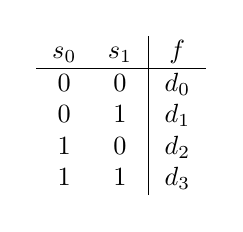
\begin{tikzpicture}
\draw (0,0) node[scale=0.95]{\begin{tabular}{cc|c}
$s_0$&$s_1$&$f$\\\hline
0&0&$d_0$\\
0&1&$d_1$\\
1&0&$d_2$\\
1&1&$d_3$
\end{tabular}};
\end{tikzpicture}
\figlab{multiplexerTruthTable}}
\subfigure[Mogelijke Implementatie]{
%\begin{tikzpicture}[circuit logic US,scale=1,xscale=0.8]
%\draw[dashed] (-3.5,2.25) -- (3.5,2.25) -- (2.25,-0.25) -- (-2.25,-0.25) -- cycle;
%\node[or gate, inputs={normal,normal,normal,normal},scale=0.7,rotate=-90] (O) at (0,0.25) {};
%\foreach\d/\dga/\dgb in {0/inverted/inverted,1/inverted/normal,2/normal/inverted,3/normal/normal} {
%  \node[and gate, inputs={\dga,\dgb,normal},scale=0.7,rotate=-90] (A\d) at (2.25-1.5*\d,1.25) {};
%  \draw (A\d.input 3) -- (A\d.input 3 |- 0,2.25);
%  \draw (A\d.input 1) -- (A\d.input 1 |- 0,1.75);
%  \draw (A\d.input 2) -- (A\d.input 2 |- 0,2);
%  \draw[dashed] (A\d.input 3 |- 0,2.25) -- ++(0,0.25) node[anchor=south]{$d_\d$};
%}
%\foreach\s/\g in {0/1,1/2} {
%  \draw[dashed] (-3-1/6-\s/6,1.75+0.25*\s) -- (-3.75,1.75+0.25*\s) node[anchor=east]{$s_\s$};
%  \draw (-3-1/6-\s/6,1.75+0.25*\s) -- (A0.input \g |- 0,1.75+0.25*\s);
%}
%\foreach\d/\g/\y in {0/1/0,1/2/1,2/3/1,3/4/0} {
%  \draw (A\d.output) -- ++(0,-0.25+\y*0.1) -| (O.input \g);
%}
%\draw (O.output) -- (O.output |- 0,-0.25);
%\draw[dashed] (O.output |- 0,-0.25) -- (O.output |- 0,-0.5) node[anchor=north]{$f$};
%\end{tikzpicture}
\begin{tikzpicture}[circuit logic US,scale=4]
\draw[dashed] (-0.5,-0.3) -- (-0.8,0.3) -- (0.8,0.3) -- (0.5,-0.3) -- cycle;
\node[or gate,scale=0.2*0.85,rotate=-90,inputs={normal,normal,normal,normal}] (O) at (0,-0.15) {};
\node[and gate,scale=0.2,rotate=-90,inputs={inverted,normal,inverted}] (A0) at (0.45,0.09) {};
\node[and gate,scale=0.2,rotate=-90,inputs={normal,normal,inverted}] (A1) at (0.16,0.09) {};
\node[and gate,scale=0.2,rotate=-90,inputs={inverted,normal,normal}] (A2) at (-0.16,0.09) {};
\node[and gate,scale=0.2,rotate=-90,inputs={normal,normal,normal}] (A3) at (-0.48,0.09) {};
\coordinate (Fdl) at (0,-0.3);
\coordinate (Sia) at (-0.6,-0.1);
\coordinate (Sib) at (-0.7,0.1);
\coordinate (Soa) at (0.6,-0.1);
\coordinate (Sob) at (0.7,0.1);
\coordinate (Dia) at (A0.output |- 0,0.3);
\coordinate (Dib) at (A1.output |- 0,0.3);
\coordinate (Dic) at (A2.output |- 0,0.3);
\coordinate (Did) at (A3.output |- 0,0.3);
\draw (Sib) |- (Sob |- 0,0.265) -- (Sob);
\draw (Sia) |- (Soa |- 0,0.225) -- (Soa);
\draw (Dia) -- (A0.input 2);
\draw (Dib) -- (A1.input 2);
\draw (Dic) -- (A2.input 2);
\draw (Did) -- (A3.input 2);
\draw[dashed] (Fdl) -- ++(0,-0.1) node[scale=0.75,anchor=north]{$f$};
\draw[dashed] (Dia) -- ++(0,0.1) node[scale=0.75,anchor=south]{$d_0$};
\draw[dashed] (Dib) -- ++(0,0.1) node[scale=0.75,anchor=south]{$d_1$};
\draw[dashed] (Dic) -- ++(0,0.1) node[scale=0.75,anchor=south]{$d_2$};
\draw[dashed] (Did) -- ++(0,0.1) node[scale=0.75,anchor=south]{$d_3$};
\draw (A0.input 1) -- (A0.input 1 |- 0,0.225);
\draw (A1.input 1) -- (A1.input 1 |- 0,0.225);
\draw (A2.input 1) -- (A2.input 1 |- 0,0.225);
\draw (A3.input 1) -- (A3.input 1 |- 0,0.225);
\draw (A0.input 3) -- (A0.input 3 |- 0,0.265);
\draw (A1.input 3) -- (A1.input 3 |- 0,0.265);
\draw (A2.input 3) -- (A2.input 3 |- 0,0.265);
\draw (A3.input 3) -- (A3.input 3 |- 0,0.265);
\draw[dashed] (Sib) -- (-0.9,0 |- Sib) node[scale=0.75,anchor=east]{$s_1$};
\draw[dashed] (Sia) -- (-0.9,0 |- Sia) node[scale=0.75,anchor=east]{$s_0$};
\draw[dashed] (Sob) -- (0.9,0 |- Sib) node[scale=0.75,anchor=west]{$s_1$};
\draw[dashed] (Soa) -- (0.9,0 |- Sia) node[scale=0.75,anchor=west]{$s_0$};
\draw (A3.output) -- (A3.output |- 0,-0.03) -| (O.input 4);
\draw (A2.output) -- (A2.output |- 0,-0.01) -| (O.input 3);
\draw (A1.output) -- (A1.output |- 0,-0.01) -| (O.input 2);
\draw (A0.output) -- (A0.output |- 0,-0.03) -| (O.input 1);
\draw (Fdl) -- (O.output);
\begin{scope}[scale=0.25]
\pdot{A0.input 1 |- 0,0.9}
\pdot{A1.input 1 |- 0,0.9}
\pdot{A2.input 1 |- 0,0.9}
\pdot{A3.input 1 |- 0,0.9}
\pdot{A0.input 3 |- 0,1.06}
\pdot{A1.input 3 |- 0,1.06}
\pdot{A2.input 3 |- 0,1.06}
\pdot{A3.input 3 |- 0,1.06}
\end{scope}
\end{tikzpicture}
\figlab{multiplexerSchema}}
\subfigure[Cascade]{
\begin{tikzpicture}[circuit logic US]
\node[mux4to1] (A) at (6,0) {};
\draw (A.selin1) -- (A.selin1 -| 1.5,0) node[scale=0.65,anchor=east]{$s_3$};
\draw (A.selin0) -- (A.selin0 -| 1.5,0) node[scale=0.65,anchor=east]{$s_2$};
\draw (A.output) -- ++(0,-0.25) node[scale=0.65,anchor=north]{$f$};
\foreach \x/\s in {0/0,1/1,2/1,3/0} {
  \node[mux4to1] (B\x) at (9-2*\x,1) {};
  \draw (B\x.output) -- ++(0,-0.25+0.125*\s) -| (A.data\x);
}
\foreach \x/\g/\i in {0/0/0,0/1/1,0/2/2,0/3/3,1/0/4,1/1/5,1/2/6,1/3/7,2/0/8,2/1/9,2/2/10,2/3/11,3/0/12,3/1/13,3/2/14,3/3/15} {
  \draw (B\x.data\g) -- ++(0,0.25) node[scale=0.65,anchor=south]{$d_{\i}$};
}
\foreach \x/\xa in {3/2,2/1,1/0} {
  \draw (B\x.selout0) -- (B\xa.selin0);
  \draw (B\x.selout1) -- (B\xa.selin1);
}
\draw (B3.selin1) -- (B3.selin1 -| 1.5,0) node[scale=0.65,anchor=east]{$s_1$};
\draw (B3.selin0) -- (B3.selin0 -| 1.5,0) node[scale=0.65,anchor=east]{$s_0$};
\end{tikzpicture}
\figlab{multiplexerCascade}}
\caption{Multiplexer.}
\figlab{multiplexer}
\end{figure}
\subsubsection{Cascade}
We kunnen uiteraard multiplexers met een verschillende parameter $n$ bouwen. Het probleem is echter dat deze waarden erg kunnen vari\"eren, wat weinig interessant is voor massaproductie. Daarom zal men veelal met een \termen{cascade} werken. Figuur \ref{fig:multiplexerCascade} toont een 16-naar-1 MUX gebouwd met behulp van 5 4-naar-1 multiplexers. We kunnen dit uiteraard veralgemenen: Indien we een $2^{n\times m}$-naar-1 multiplexer willen bouwen, kunnen we dit met $n$ niveaus van $2^m$-naar-1 multiplexers. Het aantal multiplexers die we in dat geval nodig hebben is:
\begin{equation}
\mbox{aantal multiplexers}=\displaystyle\frac{2^{n\times m}-1}{2^m-1}
\end{equation}
\subsection{Decoder}
\ssclab{decoder}
Een andere schakeling die sterk gerelateerd is aan een multiplexer is een \termen{decoder}. Een decoder beschikt over een \termen{enable-ingang $e$}, en $n$ \termen{adres-ingangen $a_i$}. De uitvoer bestaat uit $2^n$ \termen{selectie-uitgangen $s_i$}. Een decoder zal indien er een 1 aangelegd wordt op de enable-ingang $e$, een 1 op de uitgang zetten met index $A$. Hierbij staat $A$ voor de binaire waarde die voorgesteld wordt door de adres-ingangen $a_i$. In een blokschema wordt een decoder voorgesteld zoals op figuur \ref{fig:decoderInterface} door een rechthoek. In dit geval een 2-naar-4 decoder. Bovenaan staan de adres-ingangen $a_i$, aan de zijkant de enable-ingang $e$, en onderaan de uitgangen $s_i$.
\begin{figure}[hbt]
\centering
\subfigure[Interface]{
\begin{tikzpicture}
  \node[decoder2to4] (I) at (0,0) {Decoder};
  \draw[<-] (I.enable) -- ++(-0.25,0) node[scale=0.75,anchor=east]{$e$};
  \draw[->] (I.s0) -- ++(0,-0.25) node[scale=0.75,anchor=north]{$s_0$};
  \draw[->] (I.s1) -- ++(0,-0.25) node[scale=0.75,anchor=north]{$s_1$};
  \draw[->] (I.s2) -- ++(0,-0.25) node[scale=0.75,anchor=north]{$s_2$};
  \draw[->] (I.s3) -- ++(0,-0.25) node[scale=0.75,anchor=north]{$s_3$};
  \draw[<-] (I.a0) -- ++(0,0.25) node[scale=0.75,anchor=south]{$a_0$};
  \draw[<-] (I.a1) -- ++(0,0.25) node[scale=0.75,anchor=south]{$a_1$};
\end{tikzpicture}
\figlab{decoderInterface}
}
\subfigure[Waarheidstabel] {
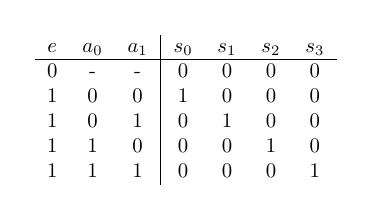
\begin{tikzpicture}
\draw (0,0) node[scale=0.75]{\begin{tabular}{ccc|cccc}
$e$&$a_0$&$a_1$&$s_0$&$s_1$&$s_2$&$s_3$\\\hline
0&-&-&0&0&0&0\\
1&0&0&1&0&0&0\\
1&0&1&0&1&0&0\\
1&1&0&0&0&1&0\\
1&1&1&0&0&0&1\\
\end{tabular}};
\end{tikzpicture}
\figlab{decoderTruthTable}}
\subfigure[Mogelijke implementatie]{
\begin{tikzpicture}[circuit logic US,scale=3]
\draw[dashed] (-0.8,-0.3) rectangle (0.8,0.3);
\draw[black!30] (0,0) node[scale=3]{Decoder};
\coordinate (Ei) at (-0.8,0);
\coordinate (Aia) at (0.26666,0.3);
\coordinate (Aib) at (-0.26666,0.3);
\coordinate (Soa) at (0.48,-0.3);
\coordinate (Sob) at (0.16,-0.3);
\coordinate (Soc) at (-0.16,-0.3);
\coordinate (Sod) at (-0.48,-0.3);
\node[and gate,scale=0.27,rotate=-90,inputs={normal,inverted,inverted},anchor=output] (A0) at (Soa |- 0,-0.25) {};
\node[and gate,scale=0.27,rotate=-90,inputs={normal,normal,inverted},anchor=output] (A1) at (Sob |- 0,-0.25) {};
\node[and gate,scale=0.27,rotate=-90,inputs={normal,inverted,normal},anchor=output] (A2) at (Soc |- 0,-0.25) {};
\node[and gate,scale=0.27,rotate=-90,inputs={normal,normal,normal},anchor=output] (A3) at (Sod |- 0,-0.25) {};
\draw (Ei) -| (-0.7,0.25) -| (A0.input 1);
\draw (A1.input 1 |- 0,0.25) -- (A1.input 1);
\draw (A2.input 1 |- 0,0.25) -- (A2.input 1);
\draw (A3.input 1 |- 0,0.25) -- (A3.input 1);
\draw (A1.input 2 |- 0,0.2) -- (A1.input 2);
\draw (A2.input 2 |- 0,0.2) -- (A2.input 2);
\draw (A1.input 3 |- 0,0.15) -- (A1.input 3);
\draw (A2.input 3 |- 0,0.15) -- (A2.input 3);
\draw (Aia) -- (Aia |- 0,0.2);
\draw (Aib) -- (Aib |- 0,0.15);
\draw (A3.input 2) -- (A3.input 2 |- 0,0.2) -| (A0.input 2);
\draw (A3.input 3) -- (A3.input 3 |- 0,0.15) -| (A0.input 3);
\draw (A0.output) -- (Soa);
\draw (A1.output) -- (Sob);
\draw (A2.output) -- (Soc);
\draw (A3.output) -- (Sod);
\draw[dashed] (Soa) -- ++(0,-0.1) node[scale=0.75,anchor=north]{$s_0$};
\draw[dashed] (Sob) -- ++(0,-0.1) node[scale=0.75,anchor=north]{$s_1$};
\draw[dashed] (Soc) -- ++(0,-0.1) node[scale=0.75,anchor=north]{$s_2$};
\draw[dashed] (Sod) -- ++(0,-0.1) node[scale=0.75,anchor=north]{$s_3$};
\draw[dashed] (Aia) -- ++(0,0.1) node[scale=0.75,anchor=south]{$a_0$};
\draw[dashed] (Aib) -- ++(0,0.1) node[scale=0.75,anchor=south]{$a_1$};
\draw[dashed] (Ei) -- ++(-0.1,0) node[scale=0.75,anchor=east]{$e$};
\begin{scope}[scale=0.333]
\pdot{A1.input 1 |- 0,0.75}
\pdot{A2.input 1 |- 0,0.75}
\pdot{A3.input 1 |- 0,0.75}
\pdot{A1.input 2 |- 0,0.6}
\pdot{A2.input 2 |- 0,0.6}
\pdot{A1.input 3 |- 0,0.45}
\pdot{A2.input 3 |- 0,0.45}
\pdot{Aia |- 0,0.6}
\pdot{Aib |- 0,0.45}
\end{scope}
\end{tikzpicture}
\figlab{decoderSchema}}
\subfigure[Cascade]{
\begin{tikzpicture}[circuit logic US]
\node[decoder2to4] (A) at (0,0) {Decoder};
\draw (A.a0) -- ++(0,0.25) node[anchor=south,scale=0.75]{$a_2$};
\draw (A.a1) -- ++(0,0.25) node[anchor=south,scale=0.75]{$a_3$};
\draw (A.enable) -- ++(-0.25,0) node[anchor=east,scale=0.75]{$e$};
\foreach\x/\y in {0/1,1/0,2/0,3/1} {
  \node[decoder2to4] (B\x) at (3-2*\x,-1.5) {Decoder};
  \draw (B\x.a0) -- ++(0,0.125) node[anchor=south,scale=0.75]{$a_0$};
  \draw (B\x.a1) -- ++(0,0.125) node[anchor=south,scale=0.75]{$a_1$};
  \draw (B\x.enable) -- ++(-0.2,0) |- (A.s\x |- 0,-0.7+0.2*\y) -- (A.s\x);
}
\foreach \x/\y/\z in {0/0/0,0/1/1,0/2/2,0/3/3,1/0/4,1/1/5,1/2/6,1/3/7,2/0/8,2/1/9,2/2/10,2/3/11,3/0/12,3/1/13,3/2/14,3/3/15} {
  \draw (B\x.s\y) -- ++(0,-0.25) node[anchor=north,scale=0.75]{$s_{\z}$};
}
\end{tikzpicture}
\figlab{decoderCascade}}
\caption{Decoder.}
\figlab{decoder}
\end{figure}
Op figuur \ref{fig:decoderTruthTable} staat de waarheidstabel voor deze component. Figuur \ref{fig:decoderSchema} toont een mogelijke implementatie. Decoders worden hoofdzakelijk gebruikt voor het decoderen van adressen.
\subsubsection{Cascade}
Net als bij multiplexer kunnen we in plaats van een heel arsenaal aan decoders aan te bieden door middel van een cascade een nieuwe decoder bouwen, zoals op figuur \ref{fig:decoderCascade}. Hier bouwen we een 4-naar-16 decoder met 5 2-naar-4 decoders. In het algemeen kunnen we een $nm$-naar-$2^{nm}$ decoder bouwen met $n$ niveaus van $m$-naar-$2^m$ decoders. In totaal hebben we dus volgend aantal decoders nodig:
\begin{equation}
\mbox{aantal decoders}=\displaystyle\frac{2^{n\times m}-1}{2^m-1}
\end{equation}
\subsubsection{Alternatieve implementatie voor Multiplexers}
Decoders worden ook gebruikt voor de synthese van bijvoorbeeld multiplexers. Figuur \ref{fig:decoderMultiplexerAnd} toont een manier om op basis van AND-poorten en een decoder een multiplexer te bouwen. We kunnen echter de OR-poort weglaten en de AND-poorten vervangen door 3-state buffers zoals op figuur \ref{fig:decoderMultiplexerTriState}. In dat geval hebben we een schakeling gerealiseerd die we een \termen{bus} noemen. Bussen zijn multiplexers waarbij we toelaten dat de ingangen gedistribueerd zijn over de verschillende delen van de schakeling. Elk van deze ingangen dienen we eenvoudigweg een uitgang van de decoder toe toe te wijzen, en de uitgang met een 3-state buffer verbinden met de bus. Bussen hebben verschillende voordelen:
\begin{itemize}
 \item We kunnen makkelijk het aantal ingangen uitbreiden. We dienen enkel over een decoder met voldoende grote $n$ te beschikken en een tri-state buffer per ingang.
 \item Indien we de traditionele Multiplexer gebruiken zal bij een groot aantal ingangen de fan-in van de OR-poort toenemen. Bovendien moeten alle ingangen van de multiplexer dicht bij elkaar staan.
 \item 3-state buffers zijn meestal gratis op een FPGA. Elk logisch blok (LB) heeft immers minstens \'e\'en uitgang langs een 3-state buffer die verbonden is met een lange lijn.
\end{itemize}
\begin{figure}[hbt]
\centering
\subfigure[Muliplexer]{
\begin{tikzpicture}[circuit logic US,scale=4]
\coordinate (Fdl) at (0,-0.3);
\coordinate (Sia) at (-0.6,-0.1);
\coordinate (Sib) at (-0.7,0.1);
\draw[dashed] (-0.5,-0.3) -- (-0.8,0.3) -- (0.8,0.3) -- (0.5,-0.3) -- cycle;
\node[decoder2to4,scale=0.75,rotate=90] (D) at (-0.50,0) {Decoder};
\draw (D.enable) -- ++(0,-0.05) node[anchor=north,scale=0.75]{$1$};
\draw (D.a0) -| (Sia);
\draw (D.a1) -- ++(-0.025,0) |- (Sib);
\node[or gate,scale=0.2*0.85,rotate=-90,inputs={normal,normal,normal,normal}] (O) at (0,-0.15) {};
\node[and gate,scale=0.2,rotate=-90,inputs={normal,normal}] (A0) at (0.24,0.09) {};
\node[and gate,scale=0.2,rotate=-90,inputs={normal,normal}] (A1) at (0.08,0.09) {};
\node[and gate,scale=0.2,rotate=-90,inputs={normal,normal}] (A2) at (-0.08,0.09) {};
\node[and gate,scale=0.2,rotate=-90,inputs={normal,normal}] (A3) at (-0.24,0.09) {};
\coordinate (Dia) at (A0.input 1 |- 0,0.3);
\coordinate (Dib) at (A1.input 1 |- 0,0.3);
\coordinate (Dic) at (A2.input 1 |- 0,0.3);
\coordinate (Did) at (A3.input 1 |- 0,0.3);
\draw (Dia) -- (A0.input 1);
\draw (Dib) -- (A1.input 1);
\draw (Dic) -- (A2.input 1);
\draw (Did) -- (A3.input 1);
\draw (A0.input 2) |- (-0.41,0.27) |- (D.s0);
\draw (A1.input 2) |- (-0.38,0.24) |- (D.s1);
\draw (A2.input 2) |- (-0.35,0.21) |- (D.s2);
\draw (A3.input 2) |- (-0.32,0.18) |- (D.s3);
\draw[dashed] (Fdl) -- ++(0,-0.1) node[scale=0.75,anchor=north]{$f$};
\draw[dashed] (Dia) -- ++(0,0.1) node[scale=0.75,anchor=south]{$d_0$};
\draw[dashed] (Dib) -- ++(0,0.1) node[scale=0.75,anchor=south]{$d_1$};
\draw[dashed] (Dic) -- ++(0,0.1) node[scale=0.75,anchor=south]{$d_2$};
\draw[dashed] (Did) -- ++(0,0.1) node[scale=0.75,anchor=south]{$d_3$};
\draw[dashed] (Sib) -- (-0.9,0 |- Sib) node[scale=0.75,anchor=east]{$s_1$};
\draw[dashed] (Sia) -- (-0.9,0 |- Sia) node[scale=0.75,anchor=east]{$s_0$};
\draw (A3.output) -- (A3.output |- 0,-0.03) -| (O.input 4);
\draw (A2.output) -- (A2.output |- 0,-0.01) -| (O.input 3);
\draw (A1.output) -- (A1.output |- 0,-0.01) -| (O.input 2);
\draw (A0.output) -- (A0.output |- 0,-0.03) -| (O.input 1);
\draw (Fdl) -- (O.output);
\end{tikzpicture}
\figlab{decoderMultiplexerAnd}}
\subfigure[Bus]{
\begin{tikzpicture}[circuit logic US,scale=4]
\coordinate (Fdl) at (0,-0.3);
\coordinate (Sia) at (-0.6,-0.1);
\coordinate (Sib) at (-0.7,0.1);
\foreach \x in {0,1,2,3} {
  \fill[black!30] (0.18-0.16*\x,0.1) rectangle (0.30-0.16*\x,-0.27);
}
\draw[dashed] (-0.5,-0.3) -- (-0.8,0.3) -- (0.8,0.3) -- (0.5,-0.3) -- cycle;
\node[decoder2to4,scale=0.75,rotate=90] (D) at (-0.50,0) {Decoder};
\draw (D.enable) -- ++(0,-0.05) node[anchor=north,scale=0.75]{$1$};
\draw (D.a0) -| (Sia);
\draw (D.a1) -- ++(-0.025,0) |- (Sib);
\node[tris,scale=0.75,rotate=-90] (T0) at (0.24,0) {};
\node[tris,scale=0.75,rotate=-90] (T1) at (0.08,0) {};
\node[tris,scale=0.75,rotate=-90] (T2) at (-0.08,0) {};
\node[tris,scale=0.75,rotate=-90] (T3) at (-0.24,0) {};
\draw (T0.z) -- (T0.z |- 0,-0.25);
\draw (T1.z) -- (T1.z |- 0,-0.25);
\draw (T2.z) -- (T2.z |- 0,-0.25);
\draw (T3.z) -- (T3.z |- 0,-0.25);
\draw (Fdl |- 0,-0.25) -- (Fdl);
\draw[thick] (T0.z |- 0,-0.25) node[anchor=west,scale=0.75]{bus} -- (T3.z |- 0,-0.25);
\coordinate (Dia) at (T0.z |- 0,0.3);
\coordinate (Dib) at (T1.z |- 0,0.3);
\coordinate (Dic) at (T2.z |- 0,0.3);
\coordinate (Did) at (T3.z |- 0,0.3);
\draw (Dia) -- (T0.x);
\draw (Dib) -- (T1.x);
\draw (Dic) -- (T2.x);
\draw (Did) -- (T3.x);
\draw (T3.c) -- (T3.c -| -0.32,0) |- (D.s3);
\foreach \x in {0,1,2} {
  \draw (T\x.c) -| (0.16-0.16*\x,0.25-0.03*\x) -| (D.s\x -| -0.41+0.03*\x,0) -- (D.s\x);
}
\draw[dashed] (Fdl) -- ++(0,-0.1) node[scale=0.75,anchor=north]{$f$};
\draw[dashed] (Dia) -- ++(0,0.1) node[scale=0.75,anchor=south]{$d_0$};
\draw[dashed] (Dib) -- ++(0,0.1) node[scale=0.75,anchor=south]{$d_1$};
\draw[dashed] (Dic) -- ++(0,0.1) node[scale=0.75,anchor=south]{$d_2$};
\draw[dashed] (Did) -- ++(0,0.1) node[scale=0.75,anchor=south]{$d_3$};
\draw[dashed] (Sib) -- (-0.9,0 |- Sib) node[scale=0.75,anchor=east]{$s_1$};
\draw[dashed] (Sia) -- (-0.9,0 |- Sia) node[scale=0.75,anchor=east]{$s_0$};
\end{tikzpicture}
\figlab{decoderMultiplexerTriState}}
\caption{Multiplexer en bus gesynthetiseerd met decoders.}
\figlab{decoderMultiplexer}
\end{figure}
\subsection{Demultiplexer}
\ssclab{demultiplexer}
Het inverse van een $2^n$-naar-1 multiplexer is een 1-naar-$2^n$ \termen{demultiplexer} (ook wel \termen{demux} genoemd). Deze component bestaat dan ook logischerwijs uit 1 \termen{data-ingang $d$} en $n$ \termen{selectie-ingangen $a_i$}. De component beschikt verder over $2^n$ uitgangen $s_i$. Logischerwijs zetten we de waarde van de data-ingang $d$ op de uitgang met de index die wordt voorgesteld door de selectie-ingangen. Een aandachtige lezer zal misschien al opgemerkt hebben dat dit probleem in wezen niet veel verschilt van de constructie van een decoder. Sterker nog, we hoeven niets aan te passen, het is alleen een kwestie van een andere interface. Figuur \ref{fig:demultiplexer} toont de interface van een demultiplexer en de equivalentie met een decoder. In tegenstelling tot de decoder zetten we de selectie-ingangen aan de zijkant en de data-ingang aan de bovenkant.
\begin{figure}[hbt]
\centering
\begin{tikzpicture}
\node[demux1to4] (DM) at (0,0) {Demux};
\draw (DM.a0) -- ++(-0.25,0) node[scale=0.75,anchor=east]{$a_0$};
\draw (DM.a1) -- ++(-0.25,0) node[scale=0.75,anchor=east]{$a_1$};
\draw (DM.s0) -- ++(0,-0.25) node[scale=0.75,anchor=north]{$s_0$};
\draw (DM.s1) -- ++(0,-0.25) node[scale=0.75,anchor=north]{$s_1$};
\draw (DM.s2) -- ++(0,-0.25) node[scale=0.75,anchor=north]{$s_2$};
\draw (DM.s3) -- ++(0,-0.25) node[scale=0.75,anchor=north]{$s_3$};
\draw (DM.data) -- ++(0,0.25) node[scale=0.75,anchor=south]{$d$};
\node (E) at (2,0) {$\equiv$};
\node[decoder2to4] (DC) at (4,0) {Decoder};
\draw (DC.a0) -- ++(0,0.25) node[scale=0.75,anchor=south]{$a_0$};
\draw (DC.a1) -- ++(0,0.25) node[scale=0.75,anchor=south]{$a_1$};
\draw (DC.s0) -- ++(0,-0.25) node[scale=0.75,anchor=north]{$s_0$};
\draw (DC.s1) -- ++(0,-0.25) node[scale=0.75,anchor=north]{$s_1$};
\draw (DC.s2) -- ++(0,-0.25) node[scale=0.75,anchor=north]{$s_2$};
\draw (DC.s3) -- ++(0,-0.25) node[scale=0.75,anchor=north]{$s_3$};
\draw (DC.enable) -- ++(-0.25,0) node[scale=0.75,anchor=east]{$d$};
\end{tikzpicture}
\caption{Demultiplexer}
\figlab{demultiplexer}
\end{figure}
\paragraph{}
Demultiplexers worden maar zeer zelden gebruikt, kun doel is immers om data op een bepaalde lijn te plaatsen, terwijl men op de andere lijnen een 0 aanlegt. In de praktijk is het aanleggen van de data op alle lijnen meestal geen probleem. In dat geval kunnen we dus de demultiplexer eenvoudigweg vervangen door een draad die de data-ingang met alle uitgangen verbindt.
\subsection{Encoder}
\label{ss:encoder}
Ook de decoder heeft een inverse: een $2^n$-naar-$n$ \termen{encoder}. Een encoder bevat $2^n$ \termen{data-ingangen $d_i$}. Het is de bedoeling dat de encoder afhankelijk van de lijn waarop een 1 staat de index weergeeft op de \termen{selectie-uitgangen $s_i$}. Verder bevat de encoder ook nog een extra uitgang: de \termen{any-uitgang $a$}, op deze uitgang wordt 1 aangelegd indien \'e\'en van de data-ingangen een 1 vertoont, anders wordt er een 0 op de any-uitgang aangelegd. We kunnen dit gedrag samenvatten in een waarheidstabel zoals in tabel \ref{tbl:truthTableEncoderNormal} voor een 4-naar-2 encoder.
\begin{table}[hbt]
\centering
\subtable[Encoder]{
\begin{tabular}{cccc|ccc}
$d_3$&$d_2$&$d_1$&$d_0$&$a$&$f_1$&$f_0$\\\hline
0&0&0&0&0&-&-\\
0&0&0&1&1&0&0\\
0&0&1&0&1&0&1\\
0&1&0&0&1&1&0\\
1&0&0&0&1&1&1\\
\end{tabular}
\tbllab{truthTableEncoderNormal}
}
\subtable[Prioriteitsencoder]{
\begin{tabular}{cccc|ccc}
$d_3$&$d_2$&$d_1$&$d_0$&$a$&$f_1$&$f_0$\\\hline
0&0&0&0&0&-&-\\
0&0&0&1&1&0&0\\
0&0&1&-&1&0&1\\
0&1&-&-&1&1&0\\
1&-&-&-&1&1&1\\
\end{tabular}
\tbllab{truthTablePriorityEncoder}
}
\caption{Waarheidtabellen van een encoder en prioriteitsencoder.}
\end{table}
Merk op dat de tabel niet alle strikt mogelijke ingangen toont. We nemen aan dat aan de ingang enkel geldige toestanden verschijnen. Indien dit niet zo is, staat het in principe vrij om elke uitgang aan te leggen. De ontbrekende rijen bevatten dus don't cares op alle uitgangen. Op basis van deze tabel kunnen we eventueel Karnaugh-kaarten maken en een implementatie voorstellen:
\begin{equation}
\left\{
\begin{array}{l}
a=d_3+d_2+d_1+d_0\\
f_1=d_3+d_1\\
f_0=d_3+d_2
\end{array}
\right.
\end{equation}
We kunnen deze schakeling dus eenvoudig realiseren met \'e\'en OR-poort per uitgang.
\paragraph{Prioriteitsencoder}
Een variant van de encoder is de \termen{prioriteitsencoder}. Een prioriteitsencoder biedt een antwoord op de ongeldige ingangen van de encoder. Hierbij telt niet d\'e index van de data-ingang waarop een 1 wordt aangelegd, maar de hoogste index van alle datalijnen met 1. Tabel \ref{tbl:truthTablePriorityEncoder} formaliseert dit. Deze schakeling kunnen we als volgt implementeren:
\begin{equation}
\left\{
\begin{array}{l}
a=d_3+d_2+d_1+d_0\\
f_1=d_3+d_2'd_1\\
f_0=d_3+d_2
\end{array}
\right.
\end{equation}
Dit komt overeen met \'e\'en extra AND- en NOT-poort. De interface voor beide schakelingen staat beschreven op figuur \ref{fig:encoderInterface}.
\begin{figure}[hbt]
\centering
\subfigure[Interfaces]{
\begin{tikzpicture}
\node[encoder4to2] (E) at (0,0) {Encoder};
\draw[<-] (E.d0) -- ++(0,0.25) node[anchor=south,scale=0.75]{$d_0$};
\draw[<-] (E.d1) -- ++(0,0.25) node[anchor=south,scale=0.75]{$d_1$};
\draw[<-] (E.d2) -- ++(0,0.25) node[anchor=south,scale=0.75]{$d_2$};
\draw[<-] (E.d3) -- ++(0,0.25) node[anchor=south,scale=0.75]{$d_3$};
\draw[->] (E.f0) -- ++(0,-0.25) node[anchor=north,scale=0.75]{$f_0$};
\draw[->] (E.f1) -- ++(0,-0.25) node[anchor=north,scale=0.75]{$f_1$};
\draw[->] (E.any) -- ++(-0.25,0) node[anchor=east,scale=0.75]{$a$};
\node[encoder4to2,text width=1.6 cm] (PE) at (3,0) {Prioriteits-encoder};
\draw[<-] (PE.d0) -- ++(0,0.25) node[anchor=south,scale=0.75]{$d_0$};
\draw[<-] (PE.d1) -- ++(0,0.25) node[anchor=south,scale=0.75]{$d_1$};
\draw[<-] (PE.d2) -- ++(0,0.25) node[anchor=south,scale=0.75]{$d_2$};
\draw[<-] (PE.d3) -- ++(0,0.25) node[anchor=south,scale=0.75]{$d_3$};
\draw[->] (PE.f0) -- ++(0,-0.25) node[anchor=north,scale=0.75]{$f_0$};
\draw[->] (PE.f1) -- ++(0,-0.25) node[anchor=north,scale=0.75]{$f_1$};
\draw[->] (PE.any) -- ++(-0.25,0) node[anchor=east,scale=0.75]{$a$};
\end{tikzpicture}
\figlab{encoderInterface}
}
\subfigure[Cascade]{
\begin{tikzpicture}
\foreach \x in {0,1,2,3} {
  \node[encoder4to2,text width=1.6 cm] (Ea\x) at (-3*\x,0) {Prioriteits-encoder};
}
\node[encoder4to2,text width=1.6 cm] (Eb3) at (-9,-3) {Prioriteits-encoder};
\node[mux4to1] (Mb2) at (-6,-3) {};
\node[mux4to1] (Mb1) at (-3,-3) {};
\foreach \x/\y/\z in {0/0/0,1/1/1,2/2/1,3/1/0} {
  \draw (Ea\x.any) -| (-3*\x-1.4,-2.4+0.1*\y) -| (Eb3.d\x);
  \draw (Ea\x.f1) -- (Ea\x.f1 |- 0,-1.6+0.1*\z) -| (Mb2.data\x);
  \draw (Ea\x.f0) -- (Ea\x.f0 |- 0,-1+0.1*\z) -| (Mb1.data\x);
}
\draw[<-] (Ea0.d0) -- ++(0,0.25) node[scale=0.75,anchor=south]{$d_0$};
\draw[<-] (Ea0.d1) -- ++(0,0.25) node[scale=0.75,anchor=south]{$d_1$};
\draw[<-] (Ea0.d2) -- ++(0,0.25) node[scale=0.75,anchor=south]{$d_2$};
\draw[<-] (Ea0.d3) -- ++(0,0.25) node[scale=0.75,anchor=south]{$d_3$};
\draw[<-] (Ea1.d0) -- ++(0,0.25) node[scale=0.75,anchor=south]{$d_4$};
\draw[<-] (Ea1.d1) -- ++(0,0.25) node[scale=0.75,anchor=south]{$d_5$};
\draw[<-] (Ea1.d2) -- ++(0,0.25) node[scale=0.75,anchor=south]{$d_6$};
\draw[<-] (Ea1.d3) -- ++(0,0.25) node[scale=0.75,anchor=south]{$d_7$};
\draw[<-] (Ea2.d0) -- ++(0,0.25) node[scale=0.75,anchor=south]{$d_8$};
\draw[<-] (Ea2.d1) -- ++(0,0.25) node[scale=0.75,anchor=south]{$d_9$};
\draw[<-] (Ea2.d2) -- ++(0,0.25) node[scale=0.75,anchor=south]{$d_{10}$};
\draw[<-] (Ea2.d3) -- ++(0,0.25) node[scale=0.75,anchor=south]{$d_{11}$};
\draw[<-] (Ea3.d0) -- ++(0,0.25) node[scale=0.75,anchor=south]{$d_{12}$};
\draw[<-] (Ea3.d1) -- ++(0,0.25) node[scale=0.75,anchor=south]{$d_{13}$};
\draw[<-] (Ea3.d2) -- ++(0,0.25) node[scale=0.75,anchor=south]{$d_{14}$};
\draw[<-] (Ea3.d3) -- ++(0,0.25) node[scale=0.75,anchor=south]{$d_{15}$};
\draw[->] (Eb3.any) -- ++(-0.25,0) node[scale=0.75,anchor=east]{$a$};
\draw[->] (Eb3.f1) -- (Eb3.f1 |- 0,-4.5) node[scale=0.75,anchor=north]{$f_3$};
\draw[->] (Eb3.f0) -- (Eb3.f0 |- 0,-4.5) node[scale=0.75,anchor=north]{$f_2$};
\draw[->] (Mb2.output) -- (Mb2.output |- 0,-4.5) node[scale=0.75,anchor=north]{$f_1$};
\draw[->] (Mb1.output) -- (Mb1.output |- 0,-4.5) node[scale=0.75,anchor=north]{$f_0$};
\draw (Eb3.f1 |- 0,-3.8) -- (-4.5,-3.8) |- (Mb1.selin1);
\draw (-7.5,-3.8) |- (Mb2.selin1);
\draw (-7.3,-4) |- (Mb2.selin0);
\draw (Eb3.f0 |- 0,-4) -- (-4.3,-4) |- (Mb1.selin0);
\pdot{Eb3.f1 |- 0,-3.8};
\pdot{-7.5,-3.8};
\pdot{-7.3,-4};
\pdot{Eb3.f0 |- 0,-4};
\end{tikzpicture}
\figlab{encoderCascade}
}
\caption{Encoder en Prioriteitsencoder.}
\end{figure}
De interface is opnieuw een rechthoek. De data-ingangen staan bovenaan, de selectie-uitgangen onderaan, en de any-uitgang aan de linkerkant.
\subsubsection{Prioriteitsencoders cascaderen}
Ook bij prioriteitsencoders gaan we even in het op het cascaderend karakter. Ook encoders laten zich eenvoudig cascaderen, mits we ook extra multiplexers gebruiken. In figuur \ref{fig:encoderCascade} bouwen we een 16-naar-4 prioriteitsencoder met 4 4-naar-2 prioriteitsencoders en 2 4-naar-1 multiplexers.

\subsection{Vergelijker}
\ssclab{comparator}
\ssclab{vergelijker}
Een \termen{vergelijker} of \termen{comparator} is een component die in staat is om uitspraken te doen over hoe twee getallen zich tot elkaar verhouden. Meestal is een vergelijker in staat om een uitspraak te doen over 4 mogelijke verhoudingen van de getallen $X$ en $Y$:
\begin{equation}
\left\{\begin{array}{c}
X<Y\\
X>Y\\
X=Y\\
X\neq Y
\end{array}\right.
\end{equation}
Op basis van de eerste twee relaties, kunnen we uitspraken doen over de laatste twee. Op basis van deze vaststelling synthetiseren we een comparator. Een comparator bevat 4 ingangen ($x_0$ ofwel $g_{\mbox{\tiny{in}}}$, $y_0$ ofwel $l_{\mbox{\tiny{in}}}$, $x_1$ en $y_1$). De twee uitgangen ($g$ en $l$) geven respectievelijk weer of het getal $X>Y$ en $X<Y$. Figuur \ref{fig:comparatorInterface} toont de interface van een vergelijker.
\begin{figure}[hbt]
\centering
\subfigure[Interface]{
\begin{tikzpicture}
\node[comp] (C) at (0,0) {Comp};
\draw[<-] (C.x0) -- ++(0.25,0) node[anchor=west,scale=0.75]{$x_0/g_{\mbox{\tiny{in}}}$};
\draw[<-] (C.y0) -- ++(0.25,0) node[anchor=west,scale=0.75]{$y_0/l_{\mbox{\tiny{in}}}$};
\draw[<-] (C.x1) -- ++(0,0.25) node[anchor=south,scale=0.75]{$x_1$};
\draw[<-] (C.y1) -- ++(0,0.25) node[anchor=south,scale=0.75]{$y_1$};
\draw[->] (C.g) -- ++(-0.25,0) node[anchor=east,scale=0.75]{$g$};
\draw[->] (C.l) -- ++(-0.25,0) node[anchor=east,scale=0.75]{$l$};
\end{tikzpicture}
\figlab{comparatorInterface}
}
\subfigure[Karnaugh-kaarten]{
\begin{tikzpicture}
\kkaartd{0}{0}{$g$}{$x_1$/$y_1$/$x_0$/$y_0$}{0/0/1/0/0/0/0/0/1/1/1/1/0/0/1/0};
\kkaartd{3}{0}{$l$}{$x_1$/$y_1$/$x_0$/$y_0$}{0/1/0/0/1/1/1/1/0/0/0/0/0/1/0/0};
\end{tikzpicture}
\figlab{comparatorKarnaugh}
}
\subfigure[Lineare cascade]{
\begin{tikzpicture}[scale=0.75]
\node[comp,scale=0.75,draw=white] (C0) at (0,0) {};
\foreach \x in {1,...,7} {
  \node[comp,scale=0.75] (C\x) at (-1.5*\x,0) {Comp};
  \draw[<-] (C\x.x1) -- ++(0,0.25) node[anchor=south,scale=0.75]{$x_{\x}$};
  \draw[<-] (C\x.y1) -- ++(0,0.25) node[anchor=south,scale=0.75]{$y_{\x}$};
}
\foreach \x/\y in {1/2,2/3,3/4,4/5,5/6,6/7} {
  \draw (C\x.g) -- (C\y.x0);
  \draw (C\x.l) -- (C\y.y0);
}
\draw[<-] (C1.x0) -| (C0.x1) -- ++(0,0.25) node[anchor=south,scale=0.75]{$x_0$};
\draw[<-] (C1.y0) -| (C0.y1) -- ++(0,0.25) node[anchor=south,scale=0.75]{$y_0$};
\draw[->] (C7.g) -- ++(-0.25,0) node[anchor=east,scale=0.75]{$g$};
\draw[->] (C7.l) -- ++(-0.25,0) node[anchor=east,scale=0.75]{$l$};
\end{tikzpicture}
\figlab{comparatorCascadeLinear}
}
\subfigure[Hi\"erarchische cascade]{
\begin{tikzpicture}[scale=0.75]
\foreach \x in {1,3,5,7} {
  \node[comp,scale=0.75] (C\x) at (-1.5*\x,0) {Comp};
  \draw[<-] (C\x.x1) -- ++(0,0.25) node[anchor=south,scale=0.75]{$x_{\x}$};
  \draw[<-] (C\x.y1) -- ++(0,0.25) node[anchor=south,scale=0.75]{$y_{\x}$};
}
\foreach \x/\y in {0/1,2/3,4/5,6/7} {
  \node[comp,scale=0.75,draw=white] (C\x) at (-1.5*\x,0) {};
  \draw[<-] (C\y.x0) -| (C\x.x1) -- ++(0,0.25) node[anchor=south,scale=0.75]{$x_{\x}$};
  \draw[<-] (C\y.y0) -| (C\x.y1) -- ++(0,0.25) node[anchor=south,scale=0.75]{$y_{\x}$};
}
\foreach \x/\y in {3/1,7/5} {
  \node[comp,scale=0.75] (Cb\x) at (-1.5*\x,-2) {Comp};
  \draw (C\x.g) -| ++(-0.4,-1.2) -| (Cb\x.x1);
  \draw (C\x.l) -| ++(-0.2,-0.6) -| (Cb\x.y1);
  \draw (C\y.g) -- ++(-0.4,0) |- (Cb\x.x0);
  \draw (C\y.l) -- ++(-0.2,0) |- (Cb\x.y0);
}
\foreach \x/\y in {7/3} {
  \node[comp,scale=0.75] (Cc\x) at (-1.5*\x,-4) {Comp};
  \draw (Cb\x.g) -| ++(-0.4,-1.2) -| (Cc\x.x1);
  \draw (Cb\x.l) -| ++(-0.2,-0.6) -| (Cc\x.y1);
  \draw (Cb\y.g) -- ++(-0.4,0) |- (Cc\x.x0);
  \draw (Cb\y.l) -- ++(-0.2,0) |- (Cc\x.y0);
}
\draw[->] (Cc7.g) -- ++(-0.25,0) node[anchor=east,scale=0.75]{$g$};
\draw[->] (Cc7.l) -- ++(-0.25,0) node[anchor=east,scale=0.75]{$l$};
\end{tikzpicture}
\figlab{comparatorCascadeHierarchical}
}
\caption{Vergelijker}
\end{figure}
Op basis van de gedragsbeschrijving kunnen we een waarheidstabel en Karnaugh-kaarten opstellen zoals op figuur \ref{fig:comparatorKarnaugh}. Op basis van deze kaarten synthetiseren we volgende formules\footnote{Merk de dualiteit op: beide formules hebben dezelfde variabelen, alleen zijn alle atomen ge\"inverteerd.}:
\begin{equation}
\left\{\begin{array}{l}
g=x_1y_1'+x_0x_1y_0'+x_0y_0'y_1'\\
l=x_1'y_1+x_0'x_1'y_0+x_0'y_0y_1
\end{array}\right.
\end{equation}
\subsubsection{Vergelijkers cascaderen}
Hoe vergelijken we nu twee getallen die uit meer dan 2-bit bestaan? Net als bij een ripple-carry opteller, kunnen we door verschillende vergelijkers aan elkaar te schakelen, een vergelijker met een groter aantal bits bouwen. In dat geval bekomen we een structuur zoals op figuur \ref{fig:comparatorCascadeLinear}. Hiermee komen we echter tot hetzelfde probleem als bij een ripple-carry opteller: de vertraging schaalt linear met het aantal bits. We kunnen echter de vergelijkers ook in een hi\"erarchische structuur kunnen we de vertraging beperken tot een logaritmische orde zoals op figuur \ref{fig:comparatorCascadeHierarchical}.
\subsubsection{Speciale gevallen}
\paragraph{Testen op gelijkheid}
We kunnen twee getallen altijd vergelijken met een vergelijker zoals eerder beschreven. Soms willen we echter twee getallen testen op specifieke eigenschappen. Bijvoorbeeld of twee getallen gelijk zijn. Dit kunnen we natuurlijk realiseren met een vergelijker, maar dit introduceert extra hardware en vertraging. In dat geval kunnen we gebruik maken van een rij van XNOR-poorten waarbij elke poort \'e\'en bit van het ene en het andere getal als invoer krijgt. De uitgangen van al deze XNOR-poorten laten we vervolgens door een OR-poort gaan. De uitvoer van deze OR poort toont ons dan of $X$ gelijk is aan $Y$. Figuur \ref{fig:comparatorEquality} toont een realisatie van dit concept voor 2 $n$-bit getallen.
\begin{figure}[hbt]
\centering
\subfigure[Gelijkheid]{
\begin{tikzpicture}[circuit logic US]
\node[and gate,inputs={normal,normal,normal,normal,normal,normal,normal},scale=0.5,rotate=-90] (O) at (-3,-1.5) {};
\node[scale=0.75] (P) at (-5,0) {$\ldots$};
\draw (O.output) -- ++(0,-0.25) node[scale=0.75,anchor=north]{$X=Y$};
\foreach \x in {0,1,2,3,4,6} {
  \coordinate (y\x) at (0.25-\x,0.75);
  \coordinate (x\x) at (-0.25-\x,0.75);
}
\foreach \x/\y/\z/\t in {0/1/3/0,1/2/2/1,2/3/1/2,3/4/0/3,4/5/1/4,6/7/3/n-1} {
  \node[xnor gate,rotate=-90] (XN\x) at (-\x,0) {};
  \draw (XN\x.input 1) -- ++(0,0.2) -| (y\x) node[scale=0.75,anchor=south]{$y_{\t}$};
  \draw (XN\x.input 2) -- ++(0,0.2) -| (x\x) node[scale=0.75,anchor=south]{$x_{\t}$};
  \draw (XN\x.output) -- ++(0,-0.1*\z) -| (O.input \y);
}
\end{tikzpicture}
\figlab{comparatorEquality}}
\subfigure[Testen met constanten]{
\begin{tikzpicture}[circuit logic US]
\node[nor gate,inputs={normal,normal,normal,normal,normal}] (O1) at (0,0) {};
\draw (O1.output) -- ++(0.25,0) node[scale=0.75,anchor=west]{$X=0$};
\node[and gate,inputs={normal,normal,normal,normal,normal}] (O2) at (0,-1.5) {};
\draw (O2.output) -- ++(0.25,0) node[scale=0.75,anchor=west]{$X=2^n-1$};
\node[not gate] (O3) at (0,-3) {};
\draw (O3.input) -- ++(-0.25,0) node[scale=0.75,anchor=east]{$x_0$};
\draw (O3.output) -- ++(0.25,0) node[scale=0.75,anchor=west]{$\mbox{even}\left(X\right)$};
\foreach \x/\t in {5/$x_0$,4/$x_1$,3/$x_2$,2/$\ldots$,1/$x_{n-1}$} {
  \draw (O1.input \x) -- ++(-0.25,0) node[scale=0.75,anchor=east]{\t};
  \draw (O2.input \x) -- ++(-0.25,0) node[scale=0.75,anchor=east]{\t};
}
\node[or gate,inputs={normal,normal,normal,normal,normal}] (O4) at (4,0) {};
\draw (O4.output) -- ++(0.25,0) node[scale=0.75,anchor=west]{$X\geq 2^k$};
\node[nand gate,inputs={normal,normal,normal,normal,normal}] (O5) at (4,-1.5) {};
\draw (O5.output) -- ++(0.25,0) node[scale=0.75,anchor=west]{$X<2^n-2^k$};
\draw (O5.output |- 0,-3) -- (O5.input 1 |- 0,-3);
\draw (O5.input 1 |- 0,-3) -- ++(-0.25,0) node[scale=0.75,anchor=east]{$x_0$};
\draw (O5.output |- 0,-3) -- ++(0.25,0) node[scale=0.75,anchor=west]{$\mbox{oneven}\left(X\right)$};
\foreach \x/\t in {5/$x_k$,4/$x_{k+1}$,3/$x_{k+2}$,2/$\ldots$,1/$x_{n-1}$} {
  \draw (O4.input \x) -- ++(-0.25,0) node[scale=0.75,anchor=east]{\t};
  \draw (O5.input \x) -- ++(-0.25,0) node[scale=0.75,anchor=east]{\t};
}
\end{tikzpicture}
\figlab{comparatorConstants}}
\caption{Speciale gevallen van vergelijkers}
\end{figure}
\paragraph{Vergelijken met constanten}
We willen een getal niet altijd vergelijken met andere getal, maar soms met een constante. In dat geval zouden we natuurlijk ook van de vergelijker kunnen gebruikmaken, en de $Y$ zelf samenstellen. Aangezien $Y$ echter op voorhand gekend is spreekt het voor zichzelf dat we de implementatie echter grondig kunnen verbeteren. Bovendien kunnen we ook testen ontwerpen die we niet kunnen uitvoeren met een vergelijker\footnote{Bijvoorbeeld deelbaarheid door 2.}. Dergelijke componenten bouwen getuigt verder ook van enig inzicht. Alle speciale gevallen beschouwen is moeilijk. Op figuur \ref{fig:comparatorConstants} geven we enkele voorbeelden.
\subsection{Schuifoperator}
\ssclab{shiftoperators}
\label{ss:shiftoperators}
Een laatste set van operaties die vaak gebruikt wordt zijn \termen{schuifoperaties}. Vele processoren implementeren schuifoperaties en bijvoorbeeld de ARM processor laat toe om tijdens elke operatie de operand over enkele plaatsen te schuiven. Een eerste probleem met schuifoperaties is dat er verschillende vormen van schuifoperaties bestaan. In het algemeen houdt een schuifoperatie in dat de waarde van de bit die eerst op plaats $i$ stond, nu op een plaats $i+m$ staat. Of formeler: $Y$ is het resultaat van een schuifoperatie van $X$ over $m$ plaatsen naar links als
\begin{equation}
\forall i\in\NN:i\in\left[0,n\right]\wedge i+m\in\left[0,n\right]\Rightarrow y_{i+m}=x_i
\end{equation}
Het probleem is wat we doen met de bits die buiten de grenzen vallen, en met wat we de nieuwe plaatsen opvullen. Voor dit probleem bestaan drie populaire oplossingen:
\begin{itemize}
 \item Bij het \termen{schuiven} negeren we de bits die buiten de grenzen vallen. Er bestaan twee vormen van schuiven die vari\"eren in wat we op de vrijgekomen plaatsen zetten:
 \begin{itemize}
   \item \termen{Logisch schuiven}: indien we logisch schuiven hebben we een extra parameter nodig, namelijk welke waarde we op de nieuwe plaatsen zetten. Soms is dit zelfs een rij van bits. We maken dus de invoer groot genoeg om geen vrije plaatsen meer over te houden.
   \item \termen{Aritmetisch schuiven}: hierbij willen we eigenlijk een wiskundige functie realiseren namelijk vermenigvuldigen of delen met een macht van 2. Hoe we dus aritmetisch schuiven hangt vooral af van de getalvoorstelling. Indien we naar links schuiven betekent dit meestal dat we de nieuwe plaatsen vullen met nullen. Indien we naar rechts schuiven zal bij een 2-complement voorstelling de hoogste bit (MSB) van het originele getal ingevoegd worden. Bij een ``unsigned'' voorstelling vullen we de vrije plaatsen ook met nullen op. Aritmetisch schuiven is vrij populair in programmeertalen. Talen die behoren tot de \verb|C/C++/C#/Java| familie introduceren daarom 2 functies: voor links (\verb+<<+) en rechts (\verb+>>+) aritmetisch schuiven deze worden gedefinieerd als:
\begin{equation}
\left\{\begin{array}{l}
X\verb+<<+M\equiv X\times 2^M\\
X\verb+>>+M\equiv X\div 2^M
\end{array}\right.
\end{equation}
 \end{itemize}
 \item Bij het \termen{roteren} vangen we de bits op die er langs \'e\'en kant afvallen en plaatsen we deze op de vrijgekomen plaatsen aan de andere kant.
\end{itemize}
\subsubsection{Implementatie van schuifoperaties}
In deze subsubsectie zullen we twee schakelingen realiseren. De eerste is een component die alle schuifoperaties kan realiseren op 4-bit getallen, maar slechts over 1 plaats naar links of rechts. Het tweede component is 8-bit \termen{barrel left rotator}. Dit component roteert 8-bit getallen naar links over een variabel aantal plaatsen. Merk op dat het bij een rotatie het eigenlijk niet uitmaakt in welke richting we roteren: een $n$-bit getal $m$ plaatsen naar links roteren is net hetzelfde als het getal $n-m$ plaatsen naar rechts roteren. Deze tweede component illustreert verder hoe we schuifoperaties effici\"ent over meerdere posities kunnen uitvoeren.
\paragraph{Schuifoperaties over 1 bit}
Indien we een component maken die meerdere operaties kan uitvoeren moeten we altijd eerst een instructieset defini\"eren, zoals in subsubsectie \ref{sss:aLUInstructionSet}. De instructieset dient zowel een onderscheid te maken tussen schuiven of roteren, aritmetisch of logisch\footnote{Enkel in geval van schuiven is dit relevant.} en links of rechts. Verder willen we ook een bit voorzien die aangeeft of er \"uberhaupt een schuifoperatie moet worden uitgevoerd. We zullen dus een 4-bit instructieset gebruiken. Tabel \ref{tbl:shiftInstructionSet} toont de betekenis van elke bit.
\begin{table}[hbt]
\centering
\begin{tabular}{c|cc}
Signaal&0&1\\\hline
$s_3$&geen schuifoperatie&schuifoperatie\\
$s_2$&links&rechts\\
$s_1$&schuiven&roteren\\
$s_0$&aritmetisch&logisch
\end{tabular}
\caption{Instructieset voor de schuifoperaties over 1 bit.}
\tbllab{shiftInstructionSet}
\end{table}
Op basis van deze instructieset kunnen we nu een component bouwen. Voor de berekening van de uitgangsbits gebruiken we multiplexers. Immers kan elke uitgang $y_i$ maar drie mogelijke uitgangen hebben: $x_{i-1}$, $x_i$ en $x_{i+1}$. Bij de uitgangen aan de rand dienen we alleen een andere interpretatie voor sommige $x_j$ te vinden. Welke van deze drie ingangen we kiezen hangt verder alleen af van twee bits uit het instructiewoord: $s_3$ en $s_2$. In het geval dat $s_3=0$ geldt $y_i=x_i$. Bijgevolg zetten we $x_i$ zowel op de $d_0$ en $d_1$ ingang van de multiplexer voor $y_i$. Indien $s_3=1$ en $s_2=0$ schuiven we naar links. We zetten dus $x_{i+1}$ en $x_{i-1}$ respectievelijk op de $d_2$ en $d_3$ ingangen. Vervolgens dienen we nog de randgevallen op te lossen. Deze randgevallen beslaan enkel $x_{i+1}$ voor $y_3$ en  $x_{i-1}$ voor $y_0$. Deze waarden zullen we respectievelijk noteren als $x_4$ en $x_{-1}$ en vallen dus buiten de grenzen van de ingangen. In geval van rotatie geldt:
\begin{equation}
\begin{array}{ll}
\left\{\begin{array}{l}
x_{-1}=x_3\\
x_4=x_0
\end{array}\right.&\mbox{(rotatie)}
\end{array}
\end{equation}
Dit dwingen we af met twee 2-naar-1 multiplexers. Deze multiplexers hebben als schakelelement instructiebit $s_1$. We dienen nu enkel nog het geval te behandelen waarin we schuiven. Indien we logisch schuiven, schuiven we de bits $L_{\mbox{\tiny{in}}}$ en $R_{\mbox{\tiny{in}}}$ in. Bij arithmetisch zullen we aan de rechterzijde een 0 inschuiven. Aan de linkerkant is dit ook het geval tenzij we schuiven met een 2-complement voorstelling. In dat laatste geval bepaalt de hoogste bit immers ook het teken van het getal. In dat geval moeten we de waarde van de hoogste bit dus nogmaals inschuiven. We kunnen bovenstaande beschrijvingen formaliseren tot volgende formules:
\begin{equation}
\begin{array}{ll}
\left\{\begin{array}{l}
x_{-1}=R_{\mbox{\tiny{in}}}\\
x_4=L_{\mbox{\tiny{in}}}
\end{array}\right.&\mbox{(schuiven, aritmetisch)}\\\\\left\{\begin{array}{l}
x_{-1}=0\\
x_4=0
\end{array}\right.&\mbox{(schuiven, logisch, unsigned)}\\\\\left\{\begin{array}{l}
x_{-1}=0\\
x_4=x_3
\end{array}\right.&\mbox{(schuiven, logisch, 2-complement)}
\end{array}
\end{equation}
Deze logica kunnen we vervolgens implementeren met OR-AND-poorten. Het resultaat van deze volledige implementatie staat op figuur \ref{fig:shiftImplementation}.
\begin{figure}[hbt]
\centering
\begin{tikzpicture}[circuit logic US]
\def\xxi{4};
\foreach \x in {0,...,3} {
  \node[mux4to1] (M\x) at (-2*\x,0) {};
  \draw (M\x.output) -- ++(0,-0.25) node[scale=0.75,anchor=north]{$y_{\x}$};
  \draw (M\x.data1) |- (M\x.data0 |- 0,0.5);
  \pdot{M\x.data0 |- 0,0.5};
  \draw (M\x.data0) -- (M\x.data0 |- 0,\xxi) node[scale=0.75,anchor=south]{$x_{\x}$};
}
\node[mux2to1] (MR) at (1.5,1.5) {};
\node[mux2to1] (ML) at (-7,1.5) {};
\draw (ML.selout0) -- (MR.selin0);
\draw (ML.selin0) -- (-8.5,0 |- ML.selin0) node[scale=0.75,anchor=east]{$s_1$};
\draw (M3.selin0) -- (-8.5,0 |- M3.selin0) node[scale=0.75,anchor=east]{$s_2$};
\draw (M3.selin1) -- (-8.5,0 |- M3.selin1) node[scale=0.75,anchor=east]{$s_3$};
\foreach \x/\y/\z in {0/1/1,1/2/0,2/3/1} {
  \draw (M\x.selin0) -- (M\y.selout0);
  \draw (M\x.selin1) -- (M\y.selout1);
  \draw (M\y.data0 |- 0,0.75) -| (M\x.data2);
  \pdot{M\y.data0 |- 0,0.75};
  \draw (M\x.data0 |- 0,1+0.25*\z) -| (M\y.data3);
  \pdot{M\x.data0 |- 0,1+0.25*\z};
}
\draw (ML.output) -- (ML.output |- 0,1) -| (M3.data2);
\draw (MR.output) -- (MR.output |- 0,1) -| (M0.data3);
\draw (ML.data1) |- (M0.data0 |- 0,1.75);
\pdot{M0.data0 |- 0,1.75};
\draw (MR.data1) |- (M3.data0 |- 0,2);
\pdot{M3.data0 |- 0,2};
\node[and gate,rotate=-90,anchor=output,scale=0.75] (AR) at (MR.data0 |- 0,2) {};
\draw (AR.output) -- (MR.data0);
\draw (AR.input 1) -- (AR.input 1 |- 0,\xxi) node[anchor=south,scale=0.75]{$R_{\mbox{\tiny{in}}}$};
\node[or gate,rotate=-90,anchor=output,scale=0.75] (OL) at (ML.data0 |- 0,1.875) {};
\draw (OL.output) -- (ML.data0);
\node[and gate,rotate=-90,anchor=north,scale=0.75] (ALa) at (OL.input 2 |- 0,3.1) {};
\node[and gate,rotate=-90,inputs={normal,normal,inverted},anchor=south,scale=0.75] (ALb) at (OL.input 1 |- 0,3.1) {};
\draw (ALa.output) -- ++(0,-0.125) -| (OL.input 2);
\draw (ALb.output) -- ++(0,-0.125) -| (OL.input 1);
\draw (ALa.input 2) |- (AR.input 2 |- 0,3.75) -- (AR.input 2);
\draw (ALa.input 2 |- 0,3.75) -- (-8.5,3.75) node[scale=0.75,anchor=east]{$s_0$};
\pdot{ALa.input 2 |- 0,3.75};
\draw (ALb.input 3 |- 0,3.75) -- (ALb.input 3);
\pdot{ALb.input 3 |- 0,3.75};
\draw (ALb.input 1) |- (M3.data0 |- 0,3.5);
\pdot{M3.data0 |- 0,3.5};
\draw (ALa.input 1) -- (ALa.input 1 |- 0,\xxi) node[anchor=south,scale=0.75]{$L_{\mbox{\tiny{in}}}$};
\draw (ALb.input 2) -- (ALb.input 2 |- 0,\xxi) node[anchor=west,scale=0.75,rotate=90]{2-comp};
\end{tikzpicture}
\caption{Implementatie van een schuifoperator over 1 bit.}
\figlab{shiftImplementation}
\end{figure}
\paragraph{8-bit barrel left rotator}
In de vorige paragraaf hebben we een schuifoperator gebouwd die 1-bit kan schuiven. Door verschillende van deze schuifoperatoren na elkaar te plaatsen kunnen we schuiven over meerdere plaatsen. Toch is dit niet erg praktisch: om $m$ plaatsen te schuiven zouden we $m$ van deze schuifoperatoren na elkaar moeten plaatsen, wat grote vertragingen zou impliceren. In deze paragraaf zullen we een rotator bouwen die de vertraging beperkt tot $\log_2 m$, met $m$ het maximaal aantal plaatsen dat kan opgeschoven worden. Het concept is echter ook toepasbaar op algemene schuifoperaties. Alleen is de implementatie te complex voor pedagogische doeleinden. Figuur \ref{fig:hBitBarrelLeftRotatorImplementation} geeft het concept mooi weer.
\begin{figure}[hbt]
\centering
\begin{tikzpicture}
\foreach \y in {0,1,2} {
  \foreach \x in {0,...,7} {
    \node[mux2to1] (M\y\x) at (-1.5*\x,1.5*\y) {};
  }
  \foreach \a/\b in {0/1,1/2,2/3,3/4,4/5,5/6,6/7} {
   \draw (M\y\b.selout0) -- (M\y\a.selin0);
  }
  \draw (M\y7.selin0) -- (M\y7.selin0 -| -11.5,0) node[scale=0.75,anchor=east]{$s_{\y}$};
}
\foreach \y/\yi in {0/1,1/2} {
  \foreach \x in {0,...,7} {
    \draw (M\yi\x.output) -- (M\y\x.data0);
    \pdot{$(M\yi\x.output)!0.25!(M\y\x.data0)$};
  }
}
\foreach \x/\xa/\xb/\xc in {0/4/2/1,1/5/3/2,2/6/4/3,3/7/5/4,4/0/6/5,5/1/7/6,6/2/0/7,7/3/1/0} {
  \draw (M2\x.data0) -- (M2\x.data0 |- 0,4.5) node[scale=0.75,anchor=south]{$x_{\x}$};
  \pdot{M2\x.data0 |- 0,4.25};
  \draw (M0\x.output) -- (M0\x.output |- 0,-0.5) node[scale=0.75,anchor=north]{$y_{\x}$};
  \draw (M2\x.data0 |- 0,4.25) -- (M2\xa.data1);
  \draw ($(M2\x.output)!0.25!(M1\x.data0)$) -- (M1\xb.data1);
  \draw ($(M1\x.output)!0.25!(M0\x.data0)$) -- (M0\xc.data1);
}
\end{tikzpicture}
\caption{Implementatie van een 8-bit barrel left rotator.}
\figlab{hBitBarrelLeftRotatorImplementation}
\end{figure}
Deze barrel left rotator is gebaseerd op het additief principe. Het additief principe stelt dat indien we een getal willen schuiven of roteren over $m$ bits, we dit ook kunnen verwezenlijken door eerst te schuiven/roteren over $m_1$ bits en vervolgens over $m_2$ bits met $m=m_1+m_2$. Indien we onze rotator bouwen volgens een structuur waarbij elke niveau $i$ een rotatie uitvoert over $2^i$ plaatsen kunnen we elke rotatie-operatie uitvoeren. Op figuur \ref{fig:hBitBarrelLeftRotatorImplementation} zien we dat het niveau $s_2$, vier plaatsen naar links roteert. Het volgende niveau twee en het laatste \'e\'en. Elk van deze niveaus heeft dezelfde vertraging. Indien we dus een $n$-bit barrel left rotator willen bouwen die maximaal $m$ plaatsen kan opschuiven moeten we dus $\left\lceil\log_2m\right\rceil$ niveaus synthetiseren. Een niveau $i$ roteert $2^i$ plaatsen voor $\forall i=0,1,\ldots,\left\lceil\log_2m\right\rceil-1$. Dit concept is eenvoudig te veralgemenen naar een volledige schuifoperator. Merk op dat het aantal niveaus dus theoretisch niet afhangt van het aantal bit in het getal. Op de meeste processoren neemt men echter $m=n$. Een andere mooie eigenschap is dat de volgorde van de niveaus niet relevant is.
